\documentclass[7pt,landscape, margin = 0.1mm]{article}
\usepackage{amssymb,amsmath,amsthm,amsfonts}
\usepackage{multicol,multirow}
\usepackage{graphicx}
\usepackage[dvipsnames]{xcolor}
% Tables
\usepackage{tabularx, multirow}
\usepackage{booktabs}
\renewcommand*{\arraystretch}{2}
\usepackage{float}
\usepackage{calc}
\usepackage{soul}
\usepackage[dvipsnames]{xcolor}
\usepackage{ifthen}
\usepackage{titlesec}
\usepackage[landscape]{geometry}
\usepackage{enumitem}
\usepackage{syntonly}
\setitemize{noitemsep,topsep=0pt,parsep=0pt,partopsep=0pt}
\usepackage[colorlinks=true,citecolor=blue,linkcolor=blue]{hyperref}
\usepackage{tikz}
\def\cm{\tikz\fill[scale=0.4](0,.35) -- (.25,0) -- (1,.7) -- (.25,.15) -- cycle;} 
\ifthenelse{\lengthtest { \paperwidth = 11in}}
    { \geometry{top=.1in,left=.1in,right=.1in,bottom=.1in} }
	{\ifthenelse{ \lengthtest{ \paperwidth = 297mm}}
		{\geometry{top=1mm,left=1mm,right=1mm,bottom=1mm} }
		{\geometry{top=1mm,left=1mm,right=1mm,bottom=1mm} }
	}

\pagestyle{empty}
\def\limn{\lim_{n\to \infty}}
\def\limxo{\lim_{x\to 0}}
\def\limxi{\lim_{x\to\infty}}
\def\limxn{\lim_{x\to-\infty}}
\def\sumk{\sum_{k=1}^\infty}
\def\sumn{\sum_{n=0}^\infty}
\def\R{\mathbb{R}}
\def\dx{\text{ d}x}
%\definecolor{col1}{rgb}{0.00, 0.03,0.45}
%\definecolor{col2}{rgb}{0.27, 0.00, 0.31}
%\definecolor{col3}{rgb}{0.32, 0.00, 0.19}
%\definecolor{col4}{rgb}{0.30, 0.00, 0.09}
%\definecolor{col5}{rgb}{0.27, 0.00, 0.01}

\makeatletter

 

\newcommand{\nextcol}{\vfill\null\columnbreak}

\newcommand{\titellinie}{\rule{1.\linewidth}{0.75pt}}

\titleformat{\subsection}
  {\normalfont\fontsize{10}{10}\bfseries}{\thesection}{1em}{}

\newcommand*{\mysection}[2][black]{\vskip 0pt \titellinie\vspace{-20pt}\section{#2}\vspace{-14pt}\titellinie \colorlet{chaptercolor}{#1}}

\newcommand*{\mysubsection}[1]{\vspace{-2mm}\color{chaptercolor}\subsection{ #1 }
\vspace{-1mm}\hrule\vspace{1.5mm}\color{black}
\vspace{2mm}}

\newcommand{\COL}[1]{ \color{chaptercolor} \bf{#1}\color{black}     \\}


\newcommand{\KRZ}[2]{\vspace{1mm} \hline \vspace{1mm} \color{chaptercolor}{RC #1}:\color{black} \   \hspace{0.2cm}\vspace{1mm}   {\begin{minipage}{20em}
#2 \end{minipage}} \vspace{1mm}  \hline \vspace{1mm}  \\}


\newcommand{\DEF}[2]{\color{chaptercolor}\bf{Def #1}:\color{black}    \hspace{0.2cm} #2 \\}

\newcommand{\NOTE}[2]{\color{chaptercolor}\bf{Note #1}:\color{black}    \hspace{0.2cm} #2 \\}

\newcommand{\COR}[2]{\color{chaptercolor}\bf{Cor #1}:\color{black}    \hspace{0.2cm} #2 \\}


\newcommand{\PROP}[2]{\color{chaptercolor}\bf{Prop #1}:\color{black}    \hspace{0.2cm} #2 \\}

\newcommand{\LEM}[2]{\color{chaptercolor}\bf{Lem #1}:\color{black}    \hspace{0.2cm} #2 \\}

\newcommand{\THE}[2]{\color{chaptercolor}\bf{Trm #1}:\color{black}    \hspace{0.2cm} #2 \\}
\newcommand{\SA}[2]{\color{chaptercolor}\bf{S #1}:\color{black}    \hspace{0.2cm} #2 \\}
\newcommand{\AX}[2]{\color{chaptercolor}\bf{Axm #1}:\color{black}    \hspace{0.2cm} #2 \\}

\newcommand{\EX}[2]{\color{chaptercolor}\bf{Ex #1}:\color{black}    \hspace{0.2cm} #2 \\}

\makeatother
\setcounter{secnumdepth}{0}
\setlength{\parindent}{0pt}
\setlength{\parskip}{0pt plus 0.5ex}
\setlength{\marginparwidth}{0pt}
\setlength{\marginparsep}{0pt}
% -----------------------------------------------------------------------
\begin{document}
\syntaxonly
\centering
\pagenumbering{arabic}
\raggedcolumns

\scriptsize

\begin{center}
     \Large{\textbf{Cheat Sheet}: Comp Sc BSc, Analysis II - Brian Funk, 21.04.2001 - \textbf{22-918-18-957}} \\
\end{center}
\begin{multicols}{4}
\setlength{\premulticols}{0.5pt}
\setlength{\postmulticols}{0.5pt}
\setlength{\multicolsep}{0.5pt}
\setlength{\columnsep}{0.2pt}
\setlength{\columnseprule}{0.4pt}

\begin{flushleft}

\mysection[red]{\centering Differentialgleichungen}


\begin{itemize}
\item $ y'(x) =  \frac {1}{a(y)}\cdot b(x) \longrightarrow$ LGSM 1
\item $G(y,y',\ldots,y^{(k)},x)$ mit $k>1 \longrightarrow$ LGSM 2
\item $y'+ay=b \longrightarrow$ LGSM 3
\item $y''+a_1y'+a_2y=b \longrightarrow$ LGSM 4
\item $y^{(k)}+a_{k-1}y^{(k-1)}+\ldots +a_{0}y=b(x) $ mit Konstanten  $a_{i} \longrightarrow$ LGSM 5
\end{itemize}





\mysubsection{LGSM 1: Separation der Variabeln}

\KRZ{Separation der Variabeln}{Sei eine ODE in der Form $$
 y'(x) =  \frac {1}{a(y)}\cdot b(x)
 $$ mit $a,b$ stetig und $a(y)\neq 0$. Dann ist die Lösung der ODE gegeben durch $$y = A^{-1}\left(B(x)+c \right)$$ wobei $A,B$ Stammfunktionen von $a,b$ sind.}
 \NOTE{Beweis}{
\begin{align*}
 & \Leftrightarrow y' &&=  \frac {1}{a(y)}\cdot b(x) \\
 & \Leftrightarrow a(y) \cdot y' &&= b(x) \\
 & \Leftrightarrow \int a(y) \cdot y'(x)dx &&= \int b(x) dx + c\\
 & \Leftrightarrow A(y) &&= B(x)+c\\
 & \Leftrightarrow y &&= A^{-1}\left(B(x)+c \right)
\end{align*}}


\EX{Separation der Variabeln}{\begin{align*}
y^{\prime}(x) & =-2 \cdot \cos (x) \cdot y(x) \\
\frac{\mathrm{d} y}{\mathrm{~d} x} & =-2 \cdot \cos (x) \cdot y \\
\int \frac{1}{y} \mathrm{~d} y & =\int-2 \cdot \cos (x) \mathrm{d} x \\
\ln (|y|) & =-2 \cdot \sin (x)+c_1 \\
|y| & =e^{-2 \cdot \sin (x)+c_1}=c_2 \cdot e^{-2 \cdot \sin (x)} \\
y(x) & =c \cdot e^{-2 \cdot \sin (x)}
\end{align*}}
\mysubsection{LGSM 2: Systemisierung}
\KRZ{ODE mit $k \geq 2$}{Eine ODE von Ordnung $k \geq 2$ lässt sich als System von $k$ ODEs von Ordnung 1 in unbekannten Funktionen $z_0,\ldots,z_{k-1}$ umschreiben. Dafür setzt man $z_{i}=y^{(i)} \forall i [0,k]$ und erhält die Bedingungen $z_{i}^{\prime}=z_{i+1}$}

\EX{ODE mit $k \geq 2$}{Die ODE \begin{align*}
\exp(y''\cdot y'+\sin(y^{x+1})) =3
\end{align*} kann umgeformt werden zu \begin{align*}
\left\{\begin{array}{l}
\exp \left(z_1^{\prime} z_1+\sin \left(z_0^{x+1}\right)\right)=3 \\
z_0^{\prime}=z_1
\end{array}\right\}
\end{align*}

}
\mysubsection{LGSM 3: Variation der Konstanten}


\KRZ{Variation der Konstanten}{
Sei $y'+ay=b$.
\begin{itemize}
\item Falls $b=0$:
Die Lösungen von der homogenen Gleichungen $$y' +ay=0$$ sind genau $$f(x)=z\cdot e^{-A(x)}$$, für $A$ eine Stammfunktion von $a$. $z\in \mathbb{C}$.

\item Falls $b\neq0$:
\begin{enumerate}
\item finde $f_{h}$ durch Fall $b=0$
\item Finde $f_{p} =e^{-A(x)}\int e^{A(x)}b(x)$
\item Die Lösung ist gegeben durch $F = \lambda f_h +f_{p}$
\end{enumerate}
\end{itemize}

}
\EX{Variation der Konstanten}{
Sei $y^{\prime}=y+x^2$ gegeben. 
\begin{enumerate}
\item Homogene ODE $y^{\prime}=y$ hat $e^x$ als Lösungsbasis.
\item Mit $a(x)=-1, b(x)=x^2$ ergibt $f_p = e^{x}\int e^{-x}x^2 =e^{x}e^{-x}\left(-x^2-2 x-2\right)=-x^2-2 x-2$
\item $f(x)=-x^2-2 x-2+\lambda \cdot e^x$ 
\end{enumerate}


}

\mysubsection{LGSM 4: Variation der Konstanten II}
Gegeben sei $y'' + a_1y'+a_{0y}=  b$
Nehme an, dass die homogene Lösung ist $f = z_1 f_1 + z_2 f_2$. Löse dafür $f_p = z_1(x) f_1 + z_2(x) f_2$, was ergibt
\begin{align*}
 z_1'(x) f_1 + z_2'(x) f_2   & = 0 \\
 z_1'(x) f_1' + z_2'(x) f_2' & = b \\
 \end{align*}



\mysubsection{LGSM 5: Charakterisches Polynom}

\KRZ{Charakterisches Polynom}{
$y^{(k)}+a_{k-1}y^{(k-1)}+\ldots +a_{0}y=b(x) $ mit Konstanten  $a_{i}$.\\
Falls $b=0$:\\
\begin{enumerate}
\item Setze $e^{\lambda x}$ in die Gleichung ein ergibt $P(t)$
\item Suche die Nullstellen $\lambda_i$ von $P(t)$ Nutze Formel: $x_{1,2}=\frac{-b \pm \sqrt{b^2-4 a c}}{2 a}$


\item Sei $k_i$  die Vielfachheit von $\lambda_i$ und $l=\operatorname{deg}(P(t))$. Die Basis ist gegeben durch:$\left\{x^{j}e^{\lambda_{i}x} \mid i \in [0,l], j \in [0,k_{i}-1] \right\}$
\item Falls Reelle Lösungen gesucht und $a_i\in \mathbb{R}$ und sei $(\l \pm m i)$ eine Nullstelle des char. Polynom. Dann gilt
$e^{lt} \left[ c_1 \cos (mt)+c_2 \sin (mt) \right] $


\end{enumerate}

Falls $b=\sum c_{i}(x)\neq 0$:\\
\begin{enumerate}
\item Berechne $f_h$
\item Nutze Superpositionsprinzip und löse $y^{(k)}+a_{k-1}y^{(k-1)}+\ldots +a_{0}y=c_{i}(x)$. Benutze dafür Educated Guess 
\item Setze Guess in Gleichung ein machen den Koeffizientenvergleich und löse das SLE. Die Lösung für den Guess ist $f_i$
\item Die Gesamtlösung ist $f=f_h + \sum f_i$ für alle Summanden von $b(x)$
\end{enumerate}


Für eine Basis $\mathcal{S}$ ist die Lösung gegeben durch $\sum_{\mathcal{S}} c_i s_i$ wobei $s_i$ Elemente aus $\mathcal{S}$ sind.


}
\mysubsection{Educated Guess}{
Falls der educated guess die gleiche Lösung ergibt wie die homogene, dann multipliziere mit $x^{m}$ wobei $m$ die Vielfacheit der Nullstelle ist.
\begin{itemize}
\item $a \cdot e^{\alpha x} \longrightarrow b \cdot e^{\alpha x} $
\item  $ a^{\star} \sin (\beta x) + b^{\star} \cos(\beta x) \longrightarrow c \sin (\beta x)+d \cos (\beta x)$
\item $P_n(x)\longrightarrow R_{n+k}(x) $ (insbesondere auch $P(x)=c$)
\item $ a e^{\alpha x} \sin (\beta x)  \longrightarrow e^{\alpha x}(c \sin (\beta x)+d \cos (\beta x))$
\item $P_n(x) e^{\alpha x}  \longrightarrow R_n(x) \cdot e^{\alpha x}$
\item $P_n(x) e^{\alpha x} \sin (\beta x)  \longrightarrow  e^{\alpha x}\left(R_n(x) \sin (\beta x)+S_n(x) \cos (\beta x)\right) $

\end{itemize}
$P_n$ sind $R_n$ sind Polynome abh. von $x$ und $k$ ist die
Ordnung der kleinsten Ableitung im homogenen Teil (LHS).
Gilt auch für $a^{\star} = 0$ oder $b^{\star} = 0$.

}
\mysubsection{Theoreme und Definitionen}

\DEF{Gewöhnliche Differentialgleichung}{
Eine Gleichung der Form 
\begin{align*}
G(y,y',\ldots,y^{(k)},x)=0
\end{align*}
 heisst gewöhnliche Differentialgleichung und $k\geq 1$ heisst \COL{Ordnung} der ODE. Ist zusätzlich $y(x_{0)}= y_{0},y'(x_{0})=y_{1}\ldots , y^{(k)}(x_0)=y_{k-1}$ mit $x_{0}, y_{0}, \ldots y_{k-1} \in \mathbb{R}$ gegeben spricht man von einem \COL{Anfangswertproblem}.
}
\NOTE{}{Lineare DFG erkennen:
\begin{itemize}
\item keine Koeffizienten vor der höchsten Ableitung
\item alle Koeffizienten sind stetige Funktionen
\item keine Produkte von y oder deren Ableitungen
\item keine Potenzen von y oder deren Ableitungen
\item keine Funktionen von y oder deren Ableitungen
\end{itemize}}

\SA{2.16: Existenz- & Eindeutigkeitssatz (kurz)}{Ein Anfangswertproblem $y'=F(y,x)$, $y(x_0)=y_{0}$ mit $F$ stetig differenzierbar hat genau eine maximale Lösung}

\SA{2.16: Existenz- & Eindeutigkeitssatz}{ Angenommen, $F: \mathbf{R}^{2} \rightarrow \mathbf{R}$ ist eine stetig differenzierbare Funktion von zwei Variablen (siehe Kapitel 3). Sei $x_{0} \in \mathbf{R}$ und $y_{0} \in \mathbf{R}$. Dann hat die gewöhnliche Differentialgleichung
 
 \begin{align*}
  y^{\prime}=F(x, y)
 \end{align*}
eine eindeutige Lösung $f$, die auf einem "größten" offenen Intervall $I$ definiert ist, das $x_{0}$ enthält und $f\left(x_{0}\right)=y_{0}$ erfüllt. Mit anderen Worten, es existiert ein Intervall $I$ und eine Funktion $f: I \rightarrow \mathbf{R}$, so dass für alle $x \in I$ gilt: $f^{\prime}(x)=F(x, f(x))$, und man kann kein größeres Intervall finden, das $I$ mit einer solchen Lösung enthält.}





\DEF{2.2.1: Lineare ODE}{Eine Lineare ODE von Ordnung $k\geq 1$ ist eine Gleichung $$y^{(k)}+ a_{k-1}y^{(k-1)}+ \ldots + a_{0}y = b $$ wobei die \COL{Koeffizienten} $a_{0}, \ldots, a_{k-1}$ und die \COL{Homogenität} $b$ Funktionen $I \to \mathbb{C}$ sind. Wobei $I \subseteq \mathbb{R}$ ein offenes Intervall ist. Eine Lösung ist eine $k$-mal differenzierbare Funktion $f:I\to \mathbb{C}$ mit $y^{(k)}+ a_{k-1}y^{(k-1)}+ \ldots + a_{0}y = b$ für alle $x \in I$.
 Falls $b=0$, heisst die Gleichung \COL{homogen} und sonst inhomogen.
 Die Gleichung $$ y^{(k)}+ a_{k-1}y^{(k-1)}+ \ldots + a_{0}y = 0$$ heisst \COL{zugehörige homogene lineare ODE} }

\NOTE{Lösungsraum}{Sind $f_1$ und $f_2$ Lösungen einer homogenen linearen ODE, so sind auch Linearkombinationen $\lambda_{1}f_{1}+ \lambda_{2}f_2$ Lösungen.}
\SA{2.23:}{Annahme: $a_{0},\ldots, a_{k-1}$ stetig. Dann gilt:
\begin{itemize}

\item  Die Lösungen der \COL{homogenen} linearen ODE bilden einen komplexen Vektorraum $S$ mit $\dim_{\mathbb{C}}S=k$
\item   Die \COL{inhomegene} ODE hat eine Lösung $f_0$. Die Menge aller Lösungen ist genau der affine Raum $f_{0}+S$
\item   Falls $y_{0},\ldots, y_{k-1}\in \mathbb{C}$: Für beliebige $x_{0}\in I$ ,  hat das Anfangswertproblem und $y(x_{0})=y_{0}$, $y\left(x_0\right)=y_0, \ldots, y^{(k-1)}\left(x_0\right)=y_{k-1}$ genau eine Lösung
\item    Falls $y_{0},\ldots, y_{k-1}\in \mathbb{R}$: $\operatorname{dim}_{\mathbb{R}}\{$ reellwertige $f \in S\}=k$, die  homogene Gleichung hat eine reellwertige Lösung $f_0$
\item   	 Die inhomegene hat die Lösung $\left\{\text{reellwertige Lösungen} \right\} = f_{0}+ \left\{ \text{reellwertige } f \in S\right\}$ 
\item   	 Für $x_0 \in I, y_0, \ldots, y_{k-1} \in \mathbb{R}$ hat das entsprechende Anfangswertproblem genau eine Lösung.

\end{itemize}}

\KRZ{Lineare ODE}{

\begin{enumerate}

\item Finde Basis $f_{1}, \ldots , f_{n}$ von S der homogenen ODE
\item Finde die partikuläre Lösung von der inhomogenen ODE. Die allgemeine Lösung ist dann $f_0+\sum_{i=1}^k \lambda_i f_i, \quad \lambda_i \in \mathbb{R} \text { oder } \mathbb{C} \text {. }$
\item Falls Anfangswertproblem: Einsetzen der Anfangswerte in die allgemeine Lösung. Das LGS für $\lambda_{1},\ldots, \lambda_{k}$ hat eine eindeutige Lösung
 
\end{enumerate}
}
\DEF{Lineare ODE mit $k=1$}{$y' +ay=b$ mit gegebenen stetigen $a,b:I\to\mathbb{C}$}

\NOTE{Linearität}{  \begin{align*}
    D                      & = \frac{d^{(k)}}{dx^k} + a_{k-1} \frac{d^{(k-1)}}{dx^{k-1}} + \dots + a_0 \\
    D(\alpha f + \beta g)  & = \alpha D(f) + \beta D(g)                                                \\
    Df_1 = b_1, Df_2 = b_2 & \Rightarrow D(f_1 + f_2) = b_1 + b_2
  \end{align*}}
  
  
\SA{Superpositionsprinzip}{
Löst $f_{0}$ die ODE mit inhomogenität $b$ und
$g_{0}$ die ODE mit inhomogenität $c$ 
Dann löst $\lambda f_{0}+ \mu g_{0}$ die ODE mit inhomogenität $\lambda b + \mu c$}

\mysection[blue]{\centering Differenzialrechnung}
\mysubsection{Stetigkeit}
\NOTE{MC}{
\begin{itemize}
\item $f$ ist differenzierbar $\Rightarrow$ $f$ ist stetig
\item  f ist differenzierbar und die Einträge der Jacobimatrix von f sind stetig $\Rightarrow$ $f$ ist stetig differenzierbar
\item  Alle Richtungsableitungen von f existieren. $\Rightarrow$ impliziert gar nichts
\item Für jedes $x_0 \in \mathbb{R}^n$ gibt es eine $m \times n$ Matrix $A$, sodass $f(x)=f\left(x_0\right)+A \cdot\left(x-x_0\right)+o\left(\left\|x-x_0\right\|\right)$. $\Leftrightarrow$   Definition von Differenzierbareit
\end{itemize}

}
\KRZ{Stetigkeit}{
\begin{enumerate}
\item Falls $f=g \star h$ mit $\star \in \left\{\circ,\cdot , \pm, \div : h\neq 0 \right\}$  und $g,h$ sind stetig dann ist $f$ stetig. Gilt auch wenn $f=(x,y)=g(x) \star h(y)$
\item Stetigkeit widerlegen: Setze alle Variabeln konstant und zeige Analog zu $\mathbb{R}$ unstetigkeit. 
\item Falls $f$ eine piecewise Funktion ist, Übergänge überprüfen mit Limes der Funktion. Benutze \COL{Prop 3.2.4} und finde zwei Folgen die nicht denselben Grenzwert haben oder zeige, dass alle Folgen den gleichen Grenzwert haben.
\end{enumerate}

}


\NOTE{Funktionen}{
\begin{itemize}

\item Injektiv: $f(x_1)=f(x_2) \Rightarrow x_1 = x_2$
\item Surjektiv: $\forall y \exists x \quad f(x)=y$

\end{itemize}
Sei $f(x)=(f_i(x),\ldots f_m(x))$ mit $f: \mathbb{R}^n \mapsto \mathbb{R}^m$ und $\forall 0\leq i \leq m f_i: \mathbb{R}^n \mapsto \mathbb{R}$ gilt 
\begin{itemize}
\item alle $f_i$ sind injektiv $\Rightarrow$ $f$ ist injektiv
\item $f$ ist surjektiv $\Rightarrow$  alle $f_i$ sind surjektiv 
\end{itemize}



}

\DEF{Norm}{Die Norm von $x \in \mathbb{R}^{n}$ ist 
$$
\left\|x \right\| =\sqrt{x_{1}^{2}+x_{2}^{2}+ \ldots +x_{n}^{2}}
$$}

\DEF{3.2.8: Stetigkeit }{$U \subseteq \mathbb{R}^{n}$,$f:U \to \mathbb{R}^{m}$ heisst stetig bei $x_{0}\in U$ falls für alle $\epsilon >0$ ein $\lambda >0$ existiert, sodass gilt:
 $$
 x \in U \quad \left\|x-x_0 \right\| < \lambda \Rightarrow \left\|f(x)-f(x_{0})\right\| < \epsilon$$
  
  Die Funktion $f$  heisst stetig, wenn es bei allen $x_{0} \in U$ stetig ist}
  
 
\DEF{3.2.1: Konvergenz einer Folge}{Eine Folge $x_{1}, x_{2}, \ldots \in \mathbb{R}^{n}$ konvergent gegen $y  \in  \mathbb{R}^{n}$ falls für alle $\epsilon > 0$ ein $N$ existiert, sodass für alle $$k\leq N \quad \left\|x_{k}-y \right\| <\epsilon $$}

\LEM{3.2.2 }{
(Die letzen zwei limes in $\mathbb{R}$ der erste in $\mathbb{R}^n$)
\begin{align*}
&\lim_{k \to \infty } x_{k}=y\\
 \iff &\lim_{k \to \infty } ||x_{k}-y||=0\\
 \iff &\lim_{k \to \infty } x_{k,l}=y_{l} \qquad (\text{für alle }1 \leq l \leq n)\\
 \end{align*}}
 
 \PROP{3.2.4}{$U \subseteq \mathbb{R}^{n}$,$f:U \to \mathbb{R}^{m}$ heisst stetig bei $x_{0}\in U \Leftrightarrow$ Für alle Folgen $x_{1},x_{2}\ldots  \in U$ mit $\lim_{k \to \infty}x_{n}=x_{0}$ gilt $\lim_{k \to \infty} f(x_{n})=f(x_{0})$}
 
 \PROP{3.2.9}{$f,g$ stetig $\Rightarrow g \circ f$ stetig}
 
 
\DEF{3.2.5: Grenzwert }{Sei $U \subseteq \mathbb{R}^n$,$f:U\to \mathbb{R}^m$. Der Grenzwert von $f$ bei $x_{0}\in U$, geschrieben  $\displaystyle \lim_{\substack{x\to x_{0}\\ x \neq x_{0}}} f(x)$, ist gleich $y$, falls für alle $\epsilon > 0$ ein $\lambda >0$ existiert, sodass gilt 
  $$
 x\in U , \quad \left\|x - x_{0} \right\|< \lambda , x \neq x_{0}\Rightarrow \left\|f(x)-y \right\| < \epsilon
 $$}

\PROP{3.2.7}{$\displaystyle \lim_{\substack{x\to x_{0}\\ x \neq x_{0}}} f(x)=y \Leftrightarrow$ Für jede Folge $x_{1}, \ldots \in U$ mit $\lim_{k \to \infty} x_{k}= x_{0}$ und $x_{k}\neq x_0$ gilt $\lim_{n\to \infty} f(x_n)=y$ }

\PROP{3.2.8}{$U \subseteq \mathbb{R}^n$,$f:U\to \mathbb{R}^m$ ist genau dann bei $x_{0} \in U$ stetig, wenn $\displaystyle \lim_{\substack{x\to x_{0}\\ x \neq x_{0}}} f(x)=f(x_0)$}

\mysubsection{Limits}

\KRZ{}{
\begin{enumerate}
\item Ausklammern und Brüche kürzen
\item Mit Polarkoordinaten ersetzen: $x=r\cos(\phi)$, $y=r\sin(\phi)$ und $x^2 +y^2 =r^2$. Falls ein Term abhängig von $\phi$ übrig bleibt $\Rightarrow$ limit undefiniert.
\item definiere $g$ so dass $|f|\leq g$ (für limits nach $0$) oder $f>/< g$ (für limits nach $\pm \infty$) und berechne $\lim g$

\end{enumerate}

}

\mysubsection{Sets}

\DEF{3.2.11}{
\begin{enumerate}
\item Eine Teilmenge \(X \subset \mathbf{R}^n\) ist \COL{beschränkt}, wenn die Menge der \(\|x\|\) für \(x \in X\) in \(\mathbf{R}\) beschränkt ist.
\item Eine Teilmenge \(X \subset \mathbf{R}^n\) ist \COL{geschlossen}, wenn für jede Folge \(\left(x_k\right)\) in \(X\), die in \(\mathbf{R}^n\) gegen einen Vektor \(y \in \mathbf{R}^n\) konvergiert, gilt: \(y \in X\).
\item Eine Teilmenge \(X \subset \mathbf{R}^n\) ist \COL{kompakt}, wenn sie beschränkt und geschlossen ist.
\item Vorlesung: Eine Teilmenge \(X \subset \mathbf{R}^n\) ist \COL{offen}, wenn für alle \(x \in U\) ein \(\delta > 0\) existiert, so dass \(\{ y \in \mathbb{R}^{n} \mid |x_{i}-y_{i}| < \delta \text{ für alle }i \}\).
\end{enumerate}
}

\NOTE{}{
\begin{itemize}
\item \COL{beschränkt}: Wenn man die Menge "überdecken" kann mit einer endlichen Form.
\item \COL{abgeschlossen}: Wenn der Rand eingeschlossen ist. $\left\{(x, y) \in \mathbb{R}^2 \mid x^2+y^2 \leq 1 \right\}$
\item \COL{nicht abgeschlossen}: Wenn der Rand nicht eingeschlossen ist $\left\{(x, y) \in \mathbb{R}^2 \mid x^2+y^2 < 1 \right\}$. $\sin(\phi)$ mit $\phi \in \mathbb{Q}$ ist auch nicht abgeschlossen. 
\item \COL{offen}: Wenn das Komplementär abgeschlossen ist und man somit immer einen "Ball" um jeden Punkt legen kann und auch dieser in der Menge ist.   
\end{itemize}
Es gilt folgendes:
\begin{itemize}
\item abgeschlossene und offene Menge sind komplemente, jedoch sind  $\varnothing, \mathbb{R}^{n}$ beides.
\item Vereinigungen $\cup$ beliebig vieler offener Mengen sind offen.
\item Durchschnitte $\cap$ beliebig vieler abgeschlossener Mengen sind abgeschlossen.
\item Der Durchschnitt $\cap$ endlich vieler offener Mengen ist offen.
\item Die Vereinigung $\cup$ endlich vieler abgeschlossener Mengen ist abgeschlossen.

\end{itemize}

}


\PROP{3.3.2}{$U \subseteq \mathbb{R}^{n} \text{ abgeschlossen} \iff \mathbb{R}^{n}\setminus U \text{ offen}$}


\PROP{3.2.13}{
Ist $f: \mathbb{R}^{n}\to \mathbb{R}^{m}$ stetig, dann:
  
  \begin{itemize}
  
 
\item $U \in \mathbb{R}^{m} \text{ offen}\implies f^{-1}(U) \subseteq \mathbb{R}^{n} \text{ offen}$
\item $U \in \mathbb{R}^{m} \text{ abgeschlossen}\implies f^{-1}(U) \subseteq \mathbb{R}^{n} \text{ abgeschlossen}$
\end{itemize}   

}

\THE{3.2.15}{Sei $X \subset \mathbf{R}^n$ eine nicht-leere kompakte Menge und $f: X \rightarrow \mathbf{R}$ eine stetige Funktion. Dann ist $f$ beschränkt und erreicht ihr Maximum und Minimum. Anders ausgedrückt existieren $x_{+}$ und $x_{-}$ in $X$, so dass
$$
f\left(x_{+}\right)=\sup _{x \in X} f(x), \quad f\left(x_{-}\right)=\inf _{x \in X} f(x) .
$$}

\mysubsection{Ableitung}
\KRZ{Hessische}{
Gegeben sei $f: \mathbb{R}^n \rightarrow \mathbb{R}$
\begin{enumerate}
\item Berechne $\nabla f =  \begin{pmatrix}
\partial_{x_{1}} f  \\
\vdots \\
\partial_{x_{n}} f  \\
\end{pmatrix} $
\item Die Hessische ist gegeben durch 
$ \begin{pmatrix}
\partial_{x_{1}} \nabla f \mid & \ldots &  \mid \partial_{x_{n}} \nabla f  \\
\end{pmatrix}$
\end{enumerate}
}
\KRZ{Dreigliedentwicklung}{
Gegeben sei eine Funktion $f: \mathbb{R}^n \mapsto \mathbb{R}$ und die Entwicklungsstelle $p_0 = (x_1,  \ldots, x_n)$
\begin{enumerate}
\item Berechne $f(p_0)$
\item Berechen $\mathcal{J}_f(p_0)$
\item Die Dreigliedentwicklung ist dann $f(p)=f(p_0)+\mathcal{J}_f(p_0) (p-p_0) + \sigma \left\| p - p_0\right\|$
\end{enumerate}

}

\KRZ{Tangentialebene}{
Gegeben sei eine Funktion $f: \mathbb{R}^2 \mapsto \mathbb{R}$ und den Punkt $p_0=(x,y)$, an welcher die Tangentialebene anliegt.

\begin{enumerate}
\item Berechne die Dreigliedentwicklung von $f(p)= C + (ax + by) + \sigma\left\| p - p_0\right\|$. Alternativ kann man auch das TP ersten Grades berechnen.
\item Ebene ist gegeben durch: 
$ \left\{ (x,y,z) \mid x,y \in \mathbb{R}, z = C + ax+by   \right\} $
\end{enumerate}
Analog kann der \COL{Tangentialraum} für $f: \mathbb{R}^n \mapsto \mathbb{R}$ berechnet werden
}

\KRZ{Beweise Differenzierbarkeit}{
Sei zu beweisen dass $f$ differenzierbar ist. 
\begin{enumerate}
\item Verwende \COL{Prop 3.4.6} um zu zeigen, dss multiplikationen und additionen von differenzierbaren Funktionen differenzierbar sind. 
\item Berechne alle partiellen Ableitungen, falls diese stetig sind folgt mit \COL{Prop 3.4.7}, dass die $f$ differenzierbar ist. 
\end{enumerate}
Falls $f$ gewisse Punkte aus dem Definitionsbereich exkludiert, können diese einfach ignoriert werden. Z.b ist $f(x, y)= \begin{cases}\frac{x^2 y}{x^4+y^2} & \text { falls }(x, y) \neq(0,0) \\ 0 & \text { falls }(x, y)=(0,0)\end{cases} $ differenzierbar. Obwohl das Limit zu $(0,0)$ divergiert.
}

\KRZ{Beweise Existenz von Richtungsableitungen}{
Sei $f$ gegeben die Stückweise definiert ist: 
$f(x, y)= \begin{cases} f_1 & \text { falls }(x, y) \neq(a,b) \\ C & \text { falls }(x, y)=(a,b)\end{cases} $
\begin{enumerate}
\item Für $(x,y)\neq(a,b)$ und alle normalen Funktionen, reicht es zu zeigen, dass alle Richtungsableitungen existieren. Mit \COL{Prop 3.4.15} folgt dann, dass alle Richtungsableitungen existieren.
\item Für $(x,y)=(a,b)$: Benutze Definition des  Limits und berechne $\lim_{t\to 0}\frac{f ((a,b)+t(u,v))}{t}$
\end{enumerate}
}

\NOTE{Kettenregel}{
$J_{g \circ f}\left(x_0\right)=J_g\left(f\left(x_0\right)\right) J_f\left(x_0\right)$
Insbesondere gilt $g\circ f = g(f(x))$}

\DEF{3.3.5}{$U \subseteq \mathbb{R}^{n}$ offen, $f:U\to \mathbb{R}$
Die $i$-te partielle Ableitung von $f$ an einem Punkt $x_{0}\in U$ ist $\partial_{x_{i}} f(x_{0}):=g'(x_{0,i})\in \mathbb{R}$, wobei $g(t)=f(x_{0,1},\dots,x_{0,i-1},t,x_{0,i+1},\dots,x_{0,n})$ mit $g: \{ t \in \mathbb{R} \mid (x_{0,1},\dots,t, \dots x_{0,n}) \in U\}\to \mathbb{R}$ falls $g$ bei $t$ differenzierbar ist.}

\DEF{3.3.9}{$U \subseteq \mathbb{R}^{n}$ offen, $f:U\to \mathbb{R}^{m}$
$f=(f_{1},\dots,f_{m})$ mit $f_{i}:U\to \mathbb{R}$
Die $m \times n$ Matrix:$$J_{f}(x)=\left(\partial x_{i}, f_{i}(x)\right)_{\substack{1 \leqslant i \leqslant m \\1 \leqslant j \leqslant n}}$$}

\DEF{3.3.11}{$U \subseteq \mathbb{R}^{n}$ offen:
     
Der \COL{Gradient} von $f:U\to \mathbb{R}$ ist:
     
 $$\text{grad } f(x) = \nabla f(x)= \left(\begin{array}{c}
     
 \partial_{x_1} f\left(x\right) \\
     
 \vdots \\
     
  \partial_{x_n} f\left(x\right)
     
  \end{array}\right)$$
  Die \COL{Divergenz} von $f:U \to \mathbb{R}^{n}$ ist:$$\text{div } f(x)=\partial x_{1}f_{1}(x)+\dots+\partial x_{n}f_{n}(x)=\text{spur}(J_{f}(x))$$}
 
\NOTE{}{$df \left( x_{0}\right)A \Leftrightarrow f$ hat die sogenannte \COL{Dreigliedentwicklung}.
$$
f(x)=f(x_{0})+A(x-x_{0})+ \operatorname{Fehler} \left(x-x_{0} \right)
$$
wobei $$\operatorname{Fehler}\left( x-x_{0}\right) = \sigma \left(||x-x_{0}|| \right) \Leftrightarrow \lim_{x \to x_{0}} \frac{\operatorname{Fehler}\left( x-x_{0}\right)}{||x-x_{0}||}=0$$} 
  
 \DEF{3.4.2}{$U \subseteq \mathbb{R}^{n}$ offen $f:U\to \mathbb{R}^{m}$ heisst \COL{differenzierbar } bei $x_{0}\in U$ falls es eine lineare Abbildung $A:\mathbb{R}^{n}\to \mathbb{R}^{m}$ sodass: $$\lim_{ x \to x_{0} } \frac{f(x)-f(x_{0})-A(x-x_{0})}{|| x-x_{0}||}=0$$}
 

\PROP{3.4.4}{Wir betrachten $U \subseteq \mathbb{R}^{n}, f: U \to \mathbb{R}^{m}$
es folgt aus $f$ ist differenzierbar dass
\begin{enumerate}


\item $f$ ist stetig
\item $\partial_{x_{j}}f_{i}$ existieren für alle $i,j$
\item Die Matrix von $\operatorname{df}\left(x_{0} \right)$ bezüglich den Standardbasen von  $\mathbb{R}^{n}$ und $\mathbb{R}^{m}$ ist gleich der Jakobimatrix $$\mathcal{J}_f (x_0 )=\begin{pmatrix}
\partial_{x_1}f_1(x_0) &  \ldots & \partial_{x_n}f_1(x_0)  \\
 \vdots &  &  \vdots \\
\partial_{x_1}f_m(x_0)  & \ldots & \partial_{x_n}f_m(x_0)  \\
\end{pmatrix}$$
\end{enumerate}

}

\PROP{3.4.6}{Sei $U \subseteq \mathbb{R}^{n}$ offen, $f,g: U \longrightarrow \mathbb{R}^{m}$ differenzierbar. Dann gilt 
\begin{enumerate}


\item $f+g$ differenzierbar und $\operatorname{d}(f+g)(x_{0})=\operatorname{df}(x_{0})+ \operatorname{d}g(x_{0})$
\item $m=1 \Rightarrow$ $f\cdot g$ differenzierbar
\item $m=1, g\neq 0$ $\frac{f}{g}$ differenzierbar
 \end{enumerate}}
 
 \PROP{3.4.7}{Wir betrachten $U \subseteq \mathbb{R}^{n}, f: U \to \mathbb{R}^{m}$
Falls $\partial_{x_{j}}f_{i}$ für alle $1\leq j\leq n$, $1\leq i \leq m$ existiert und stetig ist, dann ist $f$ differenzierbar. (Man sagt $f$ ist stetig differenzierbar)}

\PROP{3.4.9}{$U \subseteq \mathbb{R}^{n}$ offen, $V \subseteq \mathbb{R}^{m}$ offen
 $f: U \longrightarrow V, g: V \longrightarrow \mathbb{R}^{p}$ differenzierbar. Dann ist $g \circ f$ differenzierbar  und
 $$d(g\circ f)(x_{0})= dg(f(x_{0}))\circ df(x_{0})$$ Insbesondere erfüllen die Jacobimatrizen:
  $$
  \mathcal{J}_{g \circ f} (x_{0})=\mathcal{J}_{g} (f(x_{0})) \cdot \mathcal{J}_{f} (x_{0})
  $$}


\DEF{3.4.11}{$U \subseteq \mathbb{R}^{n}$ offen, $f: U \to \mathbb{R}^{m}$ differenzierbar.
 $x_{0} \in U$, $A = df(x_{0})$. Der \COL{Tangentialraum} des Graphen von $f$ bei $x_{0}$ ist der Graph von $g(x)=f(x_{0})+A(x-x_{0})$, also 
 $$ \left\{ \left(y,g(x) \right) \mid x \in \mathbb{R}^{m} \right\} \subseteq \mathbb{R}^{n}\times \mathbb{R}^{m} $$}

\DEF{3.4.13}{ Sei $U \subseteq \mathbb{R}^{m}$ offen und $f: U \longrightarrow \mathbb{R}^{m}, v\in \mathbb{R}^{m}\setminus \left\{0 \right\}, x_{0}\in U$. Die Richtungsableitung von $f$ in Richtung $v$ bei $x_{0}$:
  \begin{align*} D_{v}f(x_{0}):= \mathcal{J}_{g} (0)\in \mathbb{R}^{m} \end{align*} 
wobei  $g: \left\{ t \in \mathbb{R} \mid x_{0}+tv \in U \right\} \subseteq \mathbb{R}$
\begin{align*} g(t)=f(x_{0}+tv)\end{align*}  Es gilt  \begin{align*} \mathcal{J}_{g}=\left(\begin{array}{c}
\partial_x g_1(0) \\
\vdots \\
\partial_x g_m(0)
\end{array}\right) \end{align*} } 

\PROP{3.4.15}{$u \subseteq \mathbb{R}^n$ offen, $f: u \rightarrow \mathbb{R}^m$ stetig differenzierbar $\Rightarrow$ Für alle $x_0 \in u, v \in \mathbb{R}^n \backslash\{0\}$ gilt $\operatorname{D}_v f\left(x_0\right)=d f\left(x_0\right)(v)$ lnsbesondere$$
D_{\lambda_1 v_1+\lambda_2 V_2} f\left(x_0\right)=\lambda_1 D_{V_1} f\left(x_0\right)+\lambda_2 D_{V_2} f\left(x_0\right)
$$}

\DEF{2.5.1}{Sei $u \subseteq \mathbb{R}^n \text { offen }$ 
\begin{itemize}


\item $C^0\left(u, \mathbb{R}^m\right):=$ stetige Funktionen
\item $C^{k}\left(u, \mathbb{R}^m\right):=$ alle k-ten partiellen Ableitung existieren und sind stetig
\item $C^{\infty}\left(u, \mathbb{R}^m\right):=\bigcap_{k=0}^{\infty} C^k\left(u, \mathbb{R}^m\right)$ (glatte Funktionen)

\end{itemize}

Insbesondere ist $C^{k}$ ein Vektorraum, ein Homomorphismus und abgeschlossen unter Addition, Multiplication und Verknüpfung}
 
\DEF{3.5.9}{$u \subseteq \mathbb{R}^n \text { offen, } f: u \rightarrow \mathbb{R} c^2, x_0 \in u$ Die \COL{Hessische} von $f$ bei $x_0$ ist die $n \times m$-Matrix $$
H_f\left(x_0\right)=\left(\partial_{x_i} \partial_{x_j} f\left(x_0\right)\right)_{\substack{1 \leq i \leq n \\ 1 \leq j \leq m}}$$}

\PROP{3.5.4}{$u \subseteq \mathbb{R}^n$ offen, $f \in C^2\left(u, \mathbb{R}^m\right)$. Dann gilt$$
\partial_{x_j} \partial_{x_k} f=\partial_{x_k} \partial_{x_j} f
$$}

\KOR{}{$H_{f}(x_{0})$ ist symmetrisch}

\KOR{}{Ist $f$  $C^k$, so lassen sich $\partial_{x_{j_1}}, \ldots, \partial_{x_{j_k}}$ beliebig vertauschen}

\mysubsection{Taylorpolynome}

\KRZ{Mehrdimensionale TP}{
\begin{enumerate}
\item Berechne den Gradient $\nabla f$ ($k=1$) oder die Hessische $\mathcal{H}_f$ ($k=2$)
 \item Setze in \COL{Def 3.7.1} ein
\end{enumerate}

Alternativ kann man auch schrittweise die Taylorpolynome berechnen und dann einsetzen.
}

\EX{}{Berechne das TP von $f(x,y)=\arctan(\sin(x\cdot y))$. Es gilt $T_2(\arctan(x))=x $ und $T_2(\sin(x))=x$. Somit folgt dann $T_2(xy)=xy  \Rightarrow T_2(\sin(xy))=xy  \Rightarrow T_2(\arctan(\sin(xy)))=xy$. Oder $f(x)=\log (\frac{1}{1+x^2})$. Es gilt $T_2(\log(1-x))=-x$ und $T_2(\frac{1}{1+x^2})=1-x^2$, was $T_2(f(x)=-x^2$ ergibt.}

\DEF{3.7.1}{$f \in C^k(U, \mathbb{R})$. Dann ist das $k$-te Taylorpolynom$
 T_k f(x)=
 \sum_{\substack{m_1, \cdots, m_n \geqslant 0 \\
m_1+\ldots+m_n \leq k}} \underbrace{ \frac{1}{m_{1} ! \cdots m_{n} !} \cdot \partial_1^{m_1} \cdots \partial_n^{m_n} f\left(x_0\right) }_{\text{Konstante}}\cdot y_1^{m_1} \cdot \ldots \cdot y_n^{m_n}
$}

\NOTE{$k=1$}{\begin{align*}
f(x) & =f\left(x_0\right)+\left\langle\nabla_f\left(x_0\right), \quad y\right\rangle+\sigma(\|y\|) \\
& =\underbrace{f\left(x_0\right)+\sum_{i=1}^n \partial_i f\left(x_0\right) \cdot y_i+}_{T_{K}(1) = \text{Polynom Grad} \leq 1}\sigma(\|y\|)
\end{align*}}

\NOTE{$k=2$}{Für das zweite Taylorpolynom ergibt dass\\
$
 T_{2}f(x) = \underbrace{f(x_{0})}_{\text{ Fall 1}}+\underbrace{\left< \nabla_{f}(x_{0}, x)\right> }_{\text{Fall 2}}+ \underbrace{\sum\limits_{i=0}^{n} \frac{1}{2} \partial_{i}^{2} f(x_{0})y_{i}^{2}}_{\text{Fall 3}} 
 
 
 +\underbrace{\frac{1}{2}\sum\limits _{i=1}^{n}\sum\limits_{j=1}^{n} \partial_{i} \partial_{j} f(x_{0})\cdot y_{j}y_{i}}_{\text{Fall 4}} 
=\frac{1}{2} y^{T}H_{f}(x_{0})\cdot y$
Man berechnet alle Fälle, so dass der Grad kleiner gleich $2$ ist und somit gilt
\begin{itemize}

\item Fall 1: Alle $m_{1}\ldots m_{n}=0$ (Gesamtgrad 0)
\item Fall 2: Alle $m_{1}\ldots m_{n}=0$ ausser ein $i$ wo gilt $m_{i}=1$ (Gesamtgrad 1)
\item Fall 3: Alle $m_{1}\ldots m_{n}=0$ ausser ein $i$ wo gilt $m_{i}=2$ (Gesamtgrad 2)
\item Fall 4: Alle $m_{1}\ldots m_{n}=0$ ausser zwei $i,j$ wo gilt $m_{j}=m_{i}=1$ (Gesamtgrad 2)}

\end{itemize}

\SA{3.7.3}{$f \in C^k(u, \mathbb{R})$. Dann$$
f(x)=T_k f\left(x ; x_0\right)+\sigma\left(\|y\|^k\right) .
$$}


\mysubsection{Kritische Punkte}


\KRZ{Kritische Punkte finden}{
Sei $f:\mathbb{R}^n \to \mathbb{R}$.
\begin{enumerate}

\item Falls $\exist i \in [0,n]\lim_{x_i \to \pm \infty} f( x_0,x_1, \ldots) = \pm \infty$ hat es entweder kein minimum ($- \infty$) oder kein maximum ($+ \infty$). Gemäss \COL{TRM 3.2.15} gibt es für die anderen Fälle ein Extrempunkt.
\item Berechne Grad $\nabla_f(x_i)=0$ und finde potentielle Kandidaten für $x_i$. \colorbox{yellow!30}{Alle Kombinationen aus $x_i$}
\item Berechne Hessische $\mathcal{H}_f$ und bestimme Definitheit von $\mathcal{H}_f(x_i)$
\item Falls Funktion beschränkt: Überprüfe Ränder durch berechnen der Limites!
\end{enumerate}
}

\KRZ{Eigenwerte Finden}{
\begin{itemize}
\item[1] finde char. Polynom $\mathcal{X}_A(\lambda)= det(A-\lambda I) $
\item[2] Finde Nullstellen $\mathcal{X}_A$ 
\end{itemize}
}

\NOTE{Definitheit mit Eigenwerte}{
Aus Hermitische $\mathcal{H}_f$ folgt:
\begin{itemize}
\item  alle Eigenwerte sind positiv [negativ] $\Leftrightarrow$ Matrix ist positiv [negativ] definit.
\item Falls positive und negative Eigenwerte $\Leftrightarrow$  Matrix ist indefinit
\item Für Diagonalmatrizen sind Eigenwerte die Diagonaleinträge! 
\end{itemize} }

\NOTE{Definitheit mit Sylvester}{
Alle determinanten von oberen linken submatrizen sind strikt positiv $\Leftrightarrow$ Matrix ist positiv definit. \\
Falls Theorem stimmt mit $-A$ dann ist $A$ negativ Definit. Wichtig: Für $A \in \mathbb{R}^{n,n}$ gilt $$\operatorname{Det}(-A) =  (-1)^{n}\operatorname{Det}(A)$$ 

}

\DEF{}{$U \subseteq \mathbb{R}^M, f: U \rightarrow \mathbb{R}$. Dann heisst $x_0 \in U \ldots$

\begin{itemize}

 \item \COL{lokales Minimum} : Falls es in $\varepsilon>0$ gibt mit $\left\|x-x_0\right\|<\varepsilon, x \in U \Rightarrow f\left(x_0\right) \leqslant f(x)$
 \item \COL{lokales Maximum} : Falls es in $\varepsilon>0$ gibt mit $\left\|x-x_0\right\|<\varepsilon, x \in U \Rightarrow f\left(x_0\right) \geqslant f(x)$
\item  \COL{lokales Extremum} : falls es ein lokales Minimum oder Maximum gibt
\item \COL{globaler Extrempunkt} : falls die Bedingung für alle $x \in U$ gelten
\end{itemize}

}

\DEF{3.8.2}{$U \subseteq \mathbb{R}^n$ offen, $\quad f: u \rightarrow \mathbb{R}$ differenzierbar. $x_0 \in U$ heisst kritischer Punkt falls $\nabla f\left(x_0\right)=0$.}

\PROP{3.8.1}{$U \subseteq \mathbb{R}^n$ offen, $f: U \rightarrow \mathbb{R}$ differenzierbar.
$x_0 \in U$ lokales Extremum $\Rightarrow x_0$ kritischer Punkt}

\DEF{}{Def Eine $n \times m$ Matrix A heisst...

\begin{itemize}


\item \COL{positiv definit} $\Leftrightarrow$ für alle $y \neq 0$ gilt: $y^{\top} A y>0$
\item \COL{negativ definit} $\Leftrightarrow$für alle $y \neq 0$ gilt: $y^{\top} A y<0$
 \item \COL{indefinit} falls es $y, z$ gibt mit $y^{\top} A y<0, z^{\top} A z>0$.
 \end{itemize}}
 
 \SA{3.8.7}{$u \subseteq \mathbb{R}^m$ offen, $f: u \rightarrow \mathbb{R} C^2$, $x_0$ Kritischer Punkt. Dann:
 \begin{itemize}
 

\item $H_f\left(x_0\right)$ positiv definit $\Rightarrow x_0$ lokales Minimum.
\item $H_f\left(x_0\right)$ negativ definit $\Rightarrow x_0$ lokales Maximum
\item $H_f\left(x_0\right)$ indefinit $\Rightarrow x_0$ kein lokales Extremum
 \end{itemize}
}
\DEF{}{Ein kritischer Punkt $x_0$ von $f$ heisst \COL{degeneriert} falls $\operatorname{det} H_f\left(x_0\right)=0$}



\NOTE{}{Eigenwerte von $M$ kann man bestimmen in dem man die Gleichung $\det(M-I\lambda)$ löst.}

\NOTE{}{Es gilt für alle Punkte $x_{0}$. 
\begin{itemize}

\item $H_{f}(x_0)$ hat positive Eigenwerte $\Rightarrow$ $f$ hat kein lokales Maxima bei $x_{0}$
\item $H_{f}(x_0)$ hat negative Eigenwerte $\Rightarrow$ $f$  hat kein lokales Minima bei $x_{0}$

\end{itemize}}


\NOTE{Min-Max Satz}{
Sei $\mathcal{X} \subset \mathbb{R}^n, \mathcal{X} \neq \varnothing$ eine kompakte Menge und $f:$ $\mathcal{X} \rightarrow \mathbb{R}$ eine stetige Funktion. Dann ist $f$ beschränkt und ein Maximum $\left(x^{+}\right) /$Minimum $\left(x^{-}\right)$existieren, so dass
$$
f\left(x^{+}\right)=\sup _{x \in \mathcal{X}} f(x) \quad f\left(x^{-}\right)=\inf _{x \in \mathcal{X}} f(x)
$$}

\mysubsection{Lagrange Multiplikatoren}

\KRZ{Lagrange Multiplikatoren}{
Sei $f,g: \mathbb{R}^n \mapsto \mathbb{R}$ zwei Funktionen, wobei $g$ die Nebenbedingung ist.
\begin{enumerate}


\item Bestimme alle potentiellen Punkte $\nabla g(x_i)=0$ und überprüfe ob die Punkte $x_i$ in $g$ liegen. Falls ja $x_i$ in die Liste der potentiellen Punkte aufnehmen.
\item Stelle Gleichungssystem auf für $\nabla f\left(x_0\right)=\lambda \nabla_g\left(x_0\right)$. Es ergibt sich
\begin{itemize}
\item Eine Gleichung $\forall j \in [0,n]:  \frac{\partial f}{\partial x_j}=\frac{\partial g}{\partial x_j}$
\item Eine Gleichung für die Nebenbedingung $g(x)=0$
\end{itemize}
\item Nehme alle Lösungen des Gleichungssystems als potentielle Punkte auf.
\item Potentielle Werte überprüfen durch einsetzen.
\end{enumerate}


}

\PROP{3.9.2}{$u \leq \mathbb{R}^n$ offen, $f, g \in C^1(u, \mathbb{R})$. Falls $x_0$ lok. Extremum von $f \mid{g^{-1}(0)}$, dann $\nabla g\left(x_0\right)=0$ oder es gibt $\lambda \in \mathbb{R}$ mit $$\nabla f\left(x_0\right)=\lambda \nabla_g\left(x_0\right)$$

Wobei $f \mid{g^{-1}(0)}$ bedeutet, dass $f$ eingeschränkt ist auf $\left\{ x \in U \mid g(x)=0\right\}$}

\mysubsection{Umkehrabbildung}

\DEF{3.10.1}{ Sei $u \leq \mathbb{R}^n$ offen, $f: u \rightarrow \mathbb{R}^n$ differenzierbar. 
 $f$ heisst \COL{lokal invertierbar}  bei $x_0 \in U$ falls eine offene Menge $B$ mit $x_0 \in B$ existiert, für die gilt: $f(B) \subseteq \mathbb{R}^n$ ist offen, und es gibt ein diffbares $g: f(B) \rightarrow B$ Sodass $$f \circ g=id_{f(B)}, \quad g \circ f=i d_B$$}
 
 
 \SA{3.10.2}{Von der Umkehrabbildung $U \subseteq \mathbb{R}^n$ offen, $f: U \rightarrow \mathbb{R}^{n}$ differenzierbar. 
Falls $\operatorname{det}\left(J_f\left(x_0\right)\right) \neq 0$, dann ist $f$ lokal invertierbar bei $x_0$.
  Sei $g$ die lokale Umkehrfunktion. Dann ist
 $$
 J_g\left(f\left(x_0\right)\right)=J_f\left(x_0\right)^{-1}
 $$
 
 Falls $f\in  C^k$ ist, ist auch $g \in C^k$.}
 
 
\mysection[orange]{\centering Integralrechnung}




\mysubsection{Wegintegrale}

\KRZ{Wegintegrale}{
Gegeben sei ein Vektorfeld $V(x,y)$ und ein Weg $\gamma(t) = (\gamma_x(t) , \gamma_y(t))$ im Interval $t\in[a,b]$
\begin{enumerate}
\item Berechne $\gamma\prime =  (\gamma\prime_x(t) , \gamma\prime_y(t))^\top $
\item $$\int_a^b \left[ V(\gamma_x(t) ,\gamma_y(t)) \cdot (\gamma\prime_x(t) , \gamma\prime_y(t))^\top \right] dt $$
\end{enumerate}

}

\KRZ{Umparametrisierung}{


}


\KRZ{Konservativität widerlegen}{
\begin{itemize}
\item Kontraposition \COL{Prop 4.1.13}: $\mathcal{H}_f$ nicht symmetrisch $\Rightarrow$ $f$ nicht konservativ
 \item Zwei Parametrisierungen mit gleichen Start- Endpunkt mit unterschiedlichen Ergebnissen finden.
\end{itemize}
}

\KRZ{Potential}{
Gegeben sei ein konservatives Vektorfeld $f:\mathbb{R}^3 \rightarrow \mathbb{R}^3$ mit $f=(f_1, f_2,f_3)^\T$
Gesucht: $g: \mathbb{R}^3 \rightarrow \mathbb{R}$ mit $\nabla g=f$.

\begin{enumerate}
\item Definiere $g(x,y,z) = \int f_1 dx + a(y,z)$
\item Löse nach $a(y,z)$ in $\frac{\partial g}{\partial_y}=f_2$ und integriere $ a(y,z) = \int a(y,z) dy + b(z)$
\item Löse nach $b(z)$ in $\frac{\partial g}{\partial_z}=f_3$ und integriere $ b(z) = \int b(z)$
\end{enumerate}


}

\EX{}{

Sei $f(x, y, z)=\left(\begin{array}{l}
{\color{Blue} 9 x^2 \cos (y z)+z \sin (y)} \\
{\color{Emerald}-3 x^3 z \sin (y z)+x z \cos (y)+2 y} \\
{\color{Cyan}-3 x^3 y \sin (y z)+x \sin (y)+2 z}
\end{array}\right)$

\begin{enumerate}
\item ${\color{Blue}g_1(x, y, z)}=\int {\color{Blue}f_1 =3 x^3 \cos (y z)+x z \sin (y)} $
\item ${\color{Emerald}g_2 (y,z)} = \int \left({\color{Emerald}f_2}- { \color{Blue} \partial_y g_1(x,y,z)}\right) = \int 2y= y^2$
\item ${\color{Cyan}g_3 (z)} = \int \left({\color{Cyan}f_3}- {\color{Blue} \partial_zg_1(x,y,z)} - {\color{Emerald}\partial_z g_2(x,y)}\right) = \int 2z= z^2$
\end{enumerate}
Was dann $g={\color{Blue}g_1} + {\color{Emerald}g_2} + {\color{Cyan}g_3} = {\color{Blue}3 x^3 \cos (y z)+x z \sin (y)}+{\color{Emerald}y^2}+{\color{Cyan}z^2}+c$ ergibt

}

\DEF{4.1.1 (1)}{ $[a, b] \subseteq \mathbb{R}, f:[a, b] \rightarrow \mathbb{R}^n$ stetig.
Dann $$\int_a^b f(t) d t:=\left(\int_a^b f_1(t) d t, \ldots, \int_a^b f_n(t) d t\right) \in \mathbb{R}^n$$


}

\DEF{4.1.1 (2)}{Ein Weg ist ein stetiges $\gamma:[a, b] \rightarrow \mathbb{R}^n$. Wir betrachten nur stückweise $C^1$ Wege, d.h. es gist $k \geqslant 1$ and $a=t_0<t_1<\cdots<t_k=b$ Sodass $\left.\gamma\right|_{ \left( t_{i-1},t_{i}\right) } C^1$ für alle $1 \leq i \leq h$. Wir sagen $\gamma$ ist eir Weg von $\gamma(a)$ mach $\gamma(b)$.}

\DEF{4.1.1 (3)}{Ist $\gamma:[a, b] \rightarrow \mathbb{R}^n$ in weg, $U \subseteq \mathbb{R}^n$ sodass $\operatorname{Bild}(\gamma) \subseteq u$ und $f: U \rightarrow \mathbb{R}^n$ stetig. Dann ist das Wegintegral von $f$ entlang $\gamma$, geschrieben $\int_\gamma f(s) \cdot d \vec{s}$, definiert als
 
 $$
 \int_a^b f(\gamma(t)) \cdot \gamma^{\prime}(t) d t
 $$
 
 Skalarprodukt. Alternative Scheibweise:
 $$
 \left\langle f(\gamma(t)), \gamma^{\prime}(t)\right\rangle
 $$}

\DEF{4.1.4}{Eine \COL{orientierte Umparametrisierung} eines Wegs $\gamma:[a, b] \rightarrow \mathbb{R}^n$ ist ein Weg $\sigma:[c, d] \rightarrow \mathbb{R}^u$ mit $\sigma=\gamma \circ \varphi$, wobei $\varphi:[c, d] \rightarrow[a, b]$ stetig ist, differenzierbar auf $(c, d)$, streng monoton wachsend mit $\varphi(c)=a$ and $\varphi(d)=b$ (insbesondere bijektiv).}

\PROP{4.1.5}{$\gamma$ ein Weg in $\mathbb{R}^n$ mit einer orientierten Umparametrisierung $\sigma$ von $\gamma$ 
Sei weiter das Bild $\gamma \subseteq u \subseteq \mathbb{R}^n$ und $f: U \rightarrow \mathbb{R}^n$ stetig. Dann: $$
\int_\gamma f(s) \cdot d \vec{s}=\int_\sigma f(s) \cdot d \vec{s}
$$}

\DEF{4.1.8}{ $u \subseteq \mathbb{R}^m, \quad f: u \rightarrow \mathbb{R}^n$ stetig. Falls für alle $x_1, x_2 \in U$ das Integral
 $$
 \int_\gamma f(s) \cdot d \vec{s}
 $$
 unabhängig von der Wahl des Weges $\gamma$ von $x_1$ mach $x_2$ mit Bild $(\gamma) \subseteq U$ ist, dann ist $f$ \COL{konservativ.}}
 
 \DEF{}{$U$ heisst \COL{wegzusammenhängend} falls für alle $x, y \in U$ in Weg $\gamma$ von $x$ mach $y$ existiert mit $\operatorname{Bild}(\gamma)\subseteq U$.}
 
 \SA{4.1.10}{$u \subseteq \mathbb{R}^n$ offen, $f: u \rightarrow \mathbb{R}^n$ konservativ. Dann gibt es $\sin g \in C^1(u, \mathbb{R})$ mit $f=\nabla g$. Ein solches $g$ heisst \COL{Potential} von $f$ Falls $U$ wegzusammenhängend ist, dann is $g$ eindeutig bis auf Addition einer Konstanten.}
 
 
 \PROP{4.1.13}{$U \subseteq \mathbb{R}^n$ offen, $f: u \rightarrow \mathbb{R}^n C^1$.
$f$ konservativ $\Rightarrow \frac{\partial f_i}{\partial x_j}=\frac{\partial f_j}{\partial x_i}$ für $\quad i, j=1, \ldots, n$. $\Leftrightarrow J_f(x)$ symmetrisch für alle $x \in U$}

\SA{}{$U \subseteq \mathbb{R}^n$ offen und sternförmig, $f: U \rightarrow \mathbb{R}^n C^1$ mit $\frac{\partial f_i}{\partial x_j}=\frac{\partial f_j}{\partial x_i}$ für alle $i, j=1, \ldots, n \Rightarrow f$ konservativ}

\DEF{}{$U \subseteq \mathbb{R}^n$ heisst \COL{sternförmig} falls es ein $x_0 \in U$ gibt sodass für alle $x \in C$ die Strecke zwischen $x_0$ und $x$ in A enthalten ist.}

\NOTE{}{Es gilt Konvex $\Rightarrow$ Sternförmig $\Rightarrow$ wegzusammenhängend , da man zuerst immer zu $x_{0}$ gehen kann und dann zu einem beliebigen Punkt in $U$. }

\DEF{4.1.20}{$U \subseteq \mathbb{R}^3$ offen, $f: U \rightarrow \mathbb{R}^3 C^1$. Dann ist die Rotation das $C^0$ vektorfeld $u \rightarrow \mathbb{R}^3$ gegeben als
 $$
 \operatorname{rot}(f)=\left(\begin{array}{l}
 \partial_y f_3-\partial_z f_2 \\
 \partial_z f_1-\partial_x f_3 \\
 \partial x f_2-\partial_y f_1
 \end{array}\right)
 $$
 Es gilt $J_f(x)$ symmetrisch $\Leftrightarrow \operatorname{rot}(f)(x)=0$}

\NOTE{}{Falls Domäne sternförmig ist gilt: Feld ist konservativ$ \Leftrightarrow J_f(x)$ symmetrisch $\Leftrightarrow \operatorname{rot}(f)(x)=0$
Zusammenfassend gilt:
\begin{gather*}  
f \in C^{0}(U,\mathbb{R}^{n})\text{ konservativ mit }U \subseteq \mathbb{R}^{n}\\  
\Updownarrow\\  
f=\nabla g\text{ für }g\in C^{1}(U,\mathbb{R})\\  
\qquad\qquad\qquad\qquad \Downarrow \quad(\Uparrow\quad U \text{ sternförmig})\\  
J_{f}(x) \text{ symmetrisch}  
\end{gather*}

 }



\mysubsection{Riemannintegral}




\DEF{}{
Für $U \subseteq \mathbb{R}^n$ kompakt, $f: U \rightarrow \mathbb{R}$ stetig kann man das (Riemannintegral von $f$ auf $u \int_u f\left(x_1, \ldots, x_n\right) d x$ definieren, mit folgenden Eigenschaften:

\begin{enumerate}
\item \COL{Kompabilität} $n=1, U=[a, b] \Rightarrow \int_{[a, b]} f(x) d x=\int_a^b f(x) d x$
\item \COL{Linearität}  $\int_u a f(x)+b g(x) d x=a \int_u f(x) d x+b \int_u g(x) d x$ für $f, g: U \rightarrow \mathbb{R}$ stetig, $a, b \in \mathbb{R}$.
\item \COL{Positivität} $f \leqslant g \Rightarrow \int_u f(x) d x \leq \int_u g(x) d x$ und $f \geqslant 0, V \leq U$ kompakt $\Rightarrow \int_V f(x) d x \leq \int_U f(x) d x$
\item \COL{Dreiecksungleichung} $\left|\int_u f(x)+g(x) d x\right| \leq \int_u|f(x)| d x+\int_u|g(x)| d x$ und $\int_u f(x) d x \leqslant \int_u|f(x)| d x$	
\item \COL{Volumen} $\int_u 1 d x=\text { Volumen von } U$
\item \COL{Satz von Fubini} $n_1, n_2 \geqslant 1$ mit $n_1+n_2=n$. Sei
	$$
	\begin{aligned}
	& V\left(x_1\right)=\left\{x_2 \in \mathbb{R}^{n_2} \mid\left(x_1, x_2\right) \in U\right\} \subseteq \mathbb{R}^{n_2} \\
	& U_1=\left\{x_1 \in \mathbb{R}^{n_1} \mid V\left(x_1\right) \neq \phi\right\} \subseteq \mathbb{R}^{n_1}
	\end{aligned}
	$$
	
	Falls $g: U_1 \rightarrow \mathbb{R}, \quad g\left(x_1\right)=\int_{V\left(x_1\right)} f\left(x_1, x_2\right) d x_2$ stetig ist, dann:
	$$
	\int_u f(x) d x=\int_{u_1} \int_{V\left(x_1\right)} f(x) d x_2 d x_1
	$$
	
\item \COL{Addivität bezüglich Integrationsbereichs}: $U_1, U_2 \subseteq \mathbb{R}^n$ kompakt, $f: U_1 \cup U_2 \rightarrow \mathbb{R}$ stetig
	$
\Rightarrow \int_{u_1 \cup u_2} f(x) d x=\int_{u_1} f(x) d x+\int_{u_2} f(x) d x-\int_{u_1 \cap u_2} f(x) d x
$


\end{enumerate}



}

\DEF{4.2.3}{
\begin{enumerate}


\item  Für $1 \leqslant m \leqslant n$ ist eine parametrisierte $m$-Menge in $\mathbb{R}^n$ eine stetige Funktion
 $$
 f:\left[a_1, b_1\right] \times \cdots \times\left[a_m, b_m\right] \rightarrow \mathbb{R}^n
 $$
die $C^1$ auf $\left(a_1, b_1\right) \times \cdots \times\left(a_m, b_m\right)$ ist.
 
 \item $B \subseteq \mathbb{R}^n$ heisst  \COL{vernachlässigbar} falls
 $B \subseteq B_i / d\left(f_1\right) \cup \cdots \cup$ Bild $\left(f_k\right) \quad$ für $m_i$-Mengen $f_i$ mit $m_i<n$.
\end{enumerate}
}

\NOTE{Def 4.2.3 Informell}{ Wir können die ganze Menge mit
einer endlichen Menge an Rechtecken beliebiger
Grösse überdecken.)}
\PROP{4.2.5}{ Ist $U \subseteq \mathbb{R}^n$ kompakt und vernachlässigbar, dann $\int_u f(x) d x=0$ für alle $f \in C^0(u, \mathbb{R})$.}

\mysubsection{Uneigentliche Integrale}



\DEF{}{ $I \subseteq \mathbb{R}$ kompaktes lntervall, $a \in \mathbb{R}, f:[a, \infty) \times I \rightarrow \mathbb{R}$ stetig. Dann
 $$
 \int_{[a, \infty) \times I} f(x, y) d x d y:=\lim _{b \rightarrow \infty} \int_{[a, b] \times I} f(x, y) d x d y
 $$
Das Integral Konvergiert aber nicht, je nachdem ob der lim es tut.}



\mysubsection{Transformationsformel}

\KRZ{Transformation}{

\begin{itemize}
\item Definiere die Transformation 
$  \begin{bmatrix}
\phi_u(x,y) \\ \phi_v(x,y)
\end{bmatrix} =\begin{bmatrix}
u \\ v
\end{bmatrix} $
\item Benutze die Transformation um die Ränder des Integrals anzupassen
\item Berechne die Inverse der Transformation
$  \begin{bmatrix}
\phi_x(u,v) \\ \phi_y(u,v)
\end{bmatrix} =\begin{bmatrix}
x \\ y
\end{bmatrix} $
\item Berechne $Det = \operatorname{Det}\mathcal{}J_{\phi(u,v)^{-1}}=\operatorname{Det} \begin{bmatrix}
\partial x \phi_x & \partial y \phi_x \\
\partial x \phi_y & \partial y \phi_y \\
\end{bmatrix}$
\item Benutze die Transformationsformel mit den angepassten Rändern. \colorbox{yellow!30}{$Det$ nicht vergessen}
\end{itemize} 



} 
\KRZ{Inverse Transformation}{
Gegeben sei die Transformationsfunktion
$\phi(x,y)= ...= (\phi_u(x,y) , \phi_v(x,y)) = (u,v)^T$
Wir bekommen die Gleichungen
$\phi_u(x,y)=u (I)$ und $\phi_v(x,y)=v (II)$.



Löse  $(I)$ nach $y$ auf und Setze in $(II)$ ein $\Rightarrow$ inverse $x=..$

Löse  $(II)$ nach $x$ auf und Setze in $(I)$ ein $\Rightarrow$ inverse $y=..$

}

\KRZ{Determinante}{
Für $2\times 2$ Matrizen gilt
$$\operatorname{det}\left|\begin{array}{ll}a & c \\ b & d\end{array}\right|=a d-b c$$
Für $3 \times 3$ Matrizen nach Zeile/Reihe entwickeln und abweichslungsweise addieren/subtrahieren. (Man started bei $+$)

}

\KRZ{Standard Transformationen}{
Schreibe das Integral um entsprechend der Transformationsformel.

\begin{itemize}
\item Polar: $x= r \cos(\phi), y = r \sin(\phi)$ mit $0\leq r < \infty, 0\leq\phi < 2 \pi$ und $\det = r$
\item Elliptisch: $x= ar \cos(\phi), y = br \sin(\phi)$ mit $0\leq r < \infty, 0\leq\phi < 2 \pi$ und $\det =abr$	
\item Zylinder: $x= r \cos(\phi), y = r \sin(\phi), z=z$ mit $0\leq r,z < \infty, 0\leq\phi < 2 \pi$ und $\det = r$
\item Kugel: $x=r\sin(\phi)\cos(\theta),y=r\sin(\phi)\sin(\theta), z = r \cos(\phi)$ mit $0\leq r < \infty, 0\leq \phi < \pi, 0 \leq \theta < 2\pi$ und $\det = r^2 \sin(\phi)$
\end{itemize}








}

\DEF{}{$$
 \int_{\bar{u}} f(\varphi(x))\left|\operatorname{det} f_{\varphi}(x)\right| d x=\int_{\bar{V}} f(y) d y
$$
wobei:
\begin{itemize}

\item $\bar{u}$ kompakt, $\bar{u}=U \cup B$ für $U$ offen, $B$ vernachlässigbar
\item $\bar{V}$ kompakt, $\bar{V}=V \cup C$ für $V$ offen, $C$ vernachlässigbar
\item $\varphi: \bar{u} \rightarrow \bar{v}$ stetig, und $C^1$ auf $U$
\item $\varphi(u)=V$ and $\varphi / u$ bijektiv
\item Es gibt eine stetige Funktion $\bar{u} \rightarrow \mathbb{R}$, deren Einschränkung an $U$ gleich $\left|\operatorname{det} J_{\varphi}(x)\right|$ ist.
 \item $f: \bar{V} \rightarrow \mathbb{R}$ stetig}

\end{itemize}

\mysubsection{Schwerpunktberechnung}

\DEF{}{Der \COL{Schwerpunkt} $\bar{x}\in \mathbb{R}^{n}$ einer kompakten Menge $U \subseteq \mathbb{R}^{n}$ ist gegeben durch
 $$\bar{x_{i}}=\frac{1}{\operatorname{Vol}(U)}= \int_{U}x_{i}dx$$}

\end{flushleft}


\mysubsection{Kochrezepte Integral}

\DEF{(Akkumulationsfunktion)}{
Eine Akkumulationsfunktion ist eine Funktion in der Form:
$$ A(x) = \int_{c}^{x} f(z)dz
$$
Solange $f(z)dz$ stetig in $[c,x]$ ist gilt generell: $$A'(x)=f(x) $$
Kombiniert mit der Kettenregel folgt für eine allgemeinere Form der Funktion:
$$\frac{d}{dx} \int_{c}^{h(x)} f(z)dz = f(h(x))\cdot h'(x) = F(g(x))' $$
Ein Beispiel:
$$f(z)=\int_{0}^{x^2} \frac{1}{z^2+4}$$
hier ist $h(x)=x^2$. Somit folgt
$$\frac{d}{dx}\int_{0}^{x^2} \frac{1}{z^2+4} = \frac{1}{(x^2)^2+4}\cdot (x^2)' = \frac{2x}{x^4+4}$$
Wichtig ist anzumerken, dass die Funktion nur in der oberen Grenze eine Variabel haben kann. Falls man Funktionen in der Form $
 \int_{p(x)}^{h(x)} f(z)dz$
 antrifft kann man sie lösen indem man das Integral teilt:
 $$ \int_{p(x)}^{h(x)} f(z)dz = \int_{0}^{h(x)} f(z)dz - \int_{0}^{p(x)} f(z)dz  $$}
 
\KRZ{Unbestimmtes Integral mit Substitution}{
Man folge einfach den folgenden Schritten:
\begin{enumerate}
\item Bestimme $u := f(x)$
\item Berechne $du$ und löse für $dx$: $du = f'(x) \Rightarrow dx = \frac{du}{f'(x)}$
\item Substituiere $u$ und $du$ in die ursprüngliche Gleichung
\item Wenn sich nicht alle $x$ herauskürzen; löse für $x$ in der Gleichung des ersten Schrittes
\item Setze Schritt 4 ein.
\item Löse das Integral
\item Rücksubstituiere $x$
\end{enumerate}
Beispiel:\\
Gegeben sei $$\int x \sqrt{3x+2}dx$$
\begin{enumerate}
\item $u = 3x + 2$
\item $du = 3 \Rightarrow dx = \frac{du}{3}$
\item $\int x \sqrt{u} \frac{du}{3}$
\item $u = 3x + 2 \Rightarrow x = \frac{u-2}{3} $
\item $\int \frac{u-2}{3}\sqrt{u} \frac{du}{3}  $
\item
Die letzte Gleichung kann man relativ einfach lösen:
$$ \int \frac{u-2}{3}\sqrt{u} \frac{du}{3}   = \frac{1}{9} \int \left( u-2 \right) u^{\frac{1}{2}} du$$
$$ = \frac{1}{9} \int u^{\frac{3}{2}} - 2 u^{\frac{1}{2}} = \frac{1}{9} \left[\frac{2u^{\frac{5}{2}}}{5} - \frac{2 \cdot 2u^{\frac{3}{2}}}{3}\right]$$
$$ = \frac{2}{45}u^{\frac{5}{2}}-\frac{4}{27}u^{\frac{3}{2}}$$
\item 
$$  \frac{2}{45}u^{\frac{5}{2}}-\frac{4}{27}u^{\frac{3}{2}} = \frac{2}{45} \left[3x+2 \right]^{\frac{5}{2}}-\frac{4}{27}\left[3x+2 \right]^{\frac{3}{2}}$$
\end{enumerate}
}
\KRZ{Partielle Integration: DI-Methode}{
Gegeben sein die zu integrierenden Funktion $$\int f g$$
\begin{enumerate}
\item Wähle die zu integrierende Funktion $f$ und die zu differenzierende $g$ aus.
\item Fülle die Tabelle aus, bis:
\begin{enumerate}
\item man eine $0$ in der differenzierenden Spalte erhält
\item Eine Reihe integrierbar wird
\item Eine Reihe kommt ein zweites mal vor
\end{enumerate}
\begin{center}

\begin{tabular}{l|ll}
    & $D$ & $I$ \\ \hline
$+$   & $f$   & $g$   \\
$-$   &  $f'$ &  $\int g = g^{(-1)}$ \\ 
$+$   & $f''$  &   $g^{(-2)}$ \\ 
$\ldots$   &  &   \\ 
$\pm$ & $f^{(n)} = 0$  &  $g^{(-n)}$  \\ 
\end{tabular}
\end{center}
\item
\begin{enumerate}
\item Das Ergebnis lässt sich nun von der Tabelle ablesen, indem man die diagonalen produkte (von oben nach unten) aufsummiert. Es ergibt sich also:
$$f \cdot g^{(-1)} - f'\cdot g^{(-2)}  + \ldots  \pm f^{(n-1)}\cdot g^{(-n)}$$
\item Das Ergebnis lässt sich nun ebenfalls ablesen in dem man zuerst die diagonalen Produkte aufsummiert. Dies tut man so lange bis man zur Reihe kommt, in der das Produkt integriert werden kann. Man nehme an $f^{(n)} \cdot g^{(-n)}$ ist einfach integrierbar, dann ergibt sich:
$$ f \cdot g^{(-1)} - f'\cdot g^{(-2)}  + \ldots  \pm \int f^{(n)}\cdot g^{(-n)}$$
\item Das Ergebnis wird nun gleich berechnet wie bei (b), jedoch erhählt man eine Gleichung die man nach $\int fg$ auflösen kann.

\end{enumerate}

\end{enumerate}
}

\KRZ{Partialbruchzerlegung}{Seien $P, Q$ Polynome mit $grad(P) < grad(Q)$ und $Q$ mit der Produktzerlegung $Q(x) = \prod_{j = 1}^l \big( (x- \alpha_j)^2 + \beta_j^2\big)^{m_j} \prod_{i = 1}^k (x - \gamma_i)^{n_i}$. Dann gibt es $A_{ij}, B_{ij}, C_{ij}$ reelle Zahlen mit
$$
  \frac{P(x)}{Q(x)} = \sum_{i = 1}^l \sum_{j = 1}^{m_i} \frac{(A_{ij} + B_{ij}x)}{\big( (x- \alpha_i)^2 + \beta_i^2\big)^j} + \sum_{i = 1}^k \sum_{j = 1}^{n_i} \frac{C_{ij}}{(x-\gamma_i)^j}
$$
Bei einer Partialbruchzerlegung geht man folgendermassen vor:
\begin{enumerate}[(i)]
  \item Sei $R(x) = \frac{P(x)}{Q(x)}$. Falls $grad(P) \geq grad(Q)$ wenden wir Polynomdivision an.
  \item $Q$ lässt sich nun als $Q(x) = \prod_{j = 1}^l \big( (x- \alpha_j)^2 + \beta_j^2\big)^{m_j} \prod_{i = 1}^k (x - \gamma_i)^{n_i}$ zerlegen. Das sind
  die Komplexen und reelen Nullstellen mit ihrer vielfachheit.
  \item Wir bilden nun die "hässliche" Summe von oben
  \item Wir bestimmen mithilfe von Koeffizientenvergleich (Nennerpolynom Multiplizieren) die unbekannten $A_{ij}, B_{ij}, C_{ij}$.
\end{enumerate}
Hier ein einfaches Beispiel:
\begin{align*}
  &\frac{5x + 1}{x^2 + x - 2} = \frac{5x + 1}{(x - 1)(x + 2)} = \frac{A}{x - 1} + \frac{B}{x + 2}\\ \\
  &\Rightarrow \text{ Löse } 5x + 1 = A(x + 2) + B(x - 1)\\ \\
  &\Rightarrow \text{Setze } x = -2,\;1
\end{align*}
Mit mehreren Linearen Faktoren:
\begin{align*}
  &\frac{-2x^2 + x + 8}{x (x-2)^2} = \frac{A}{x} + \frac{B}{x - 2} + \frac{C}{(x-2)^2}\\ \\
  &\Rightarrow \text{ Löse } -2x^2 + x + 8 = A(x - 2)^2 + Bx(x - 2) + Cx
\end{align*}
Ohne reelle Nullstellen:
\begin{align*}
  &\frac{2x^2 -3x + 3}{(x-1)(x^2 + 1)} = \frac{A}{x - 1} + \frac{Bx + C}{x^2 + 1}\\ \\
  &\Rightarrow \text{ Löse } 2x^2 -3x + 3 = A(x^2 + 1) + (Bx + C)(x - 1)\\ \\
  &\Rightarrow \text{Setze } x = 0,\;1,\;2
\end{align*}}
\KRZ{Rationale Funktionen Integrieren}{
Wir betrachten einen Spezialfall der Partialbruchzerlegung.
Gegeben sei eine rationale Funktion $f(x)=\frac{P(x)}{Q(x)}$. Wir nehmen an das $deg(Q(x))=1$ und sich damit $Q(x)$ schreiben lässt als $(x - \alpha)$. Wir wollen $\int \frac{P(x)}{Q(x)}$ berechnen
\begin{enumerate}
\item Führe Polynomdivision $\frac{P(x)}{(x- \alpha)}$ aus. Wir nennen den Quotienten $q$ und den Rest $r$ wobei $deg(r)=0$
\item Schreibe um zu: $$\int\frac{P(x)}{Q(x)} = \int \frac{q (x-\alpha)}{(x-\alpha)}+ \int \frac{r}{(x-\alpha)}$$
\item Kürze und Integriere Separat: $$ \int \frac{q (x-\alpha)}{(x-\alpha)}+ \int \frac{r}{(x-\alpha)}= \int q  + r \int \frac{1}{(x-\alpha)}$$
 \item Es gelten generell: $$\int \frac{a}{x+b} dx = a \cdot \ln |x+b| $$ $$  \int (ax + b) dx = \frac{ax^2}{2	}+bx$$
\end{enumerate}
Hier ein Beispiel:

$$\int \frac{x^2-6x+8}{x+1}$$
\begin{enumerate}
\item $$(x^2-6x+8){x+1} = (x-7), r = -15$$
\item $$ \ldots = \int \frac{(x+1)(x-7)}{(x+1)} + \int \frac{-15}{(x-1)}$$
\item $$\ldots= \int (x-7) - \int \frac{1}{(x+1)}$$
\end{enumerate}
}


\section{Anhang}
\subsection{Trigonometrie}
\vspace{1mm} \hline \vspace{3 mm}
\subsubsection{Periodizität}
\begin{itemize}
 \item $\sin(\alpha + 2 \pi) = \sin(\alpha) \quad \cos(\alpha + 2 \pi) = \cos(\alpha)$
 \item $\tan(\alpha + \pi) = \tan(\alpha) \quad \cot(\alpha + \pi) = \cot(\alpha)$

\end{itemize}

\subsubsection{Parität}
\begin{itemize}
 \item $\sin(-\alpha) = - \sin(\alpha) \quad \cos(-\alpha) = \cos(\alpha)$
 \item $\tan(-\alpha) = - \tan(\alpha) \quad \cot(-\alpha) = - \cot(\alpha)$
\end{itemize}

\subsubsection{Ergänzung}
\begin{itemize}
 \item $\sin(\pi - \alpha) = \sin(\alpha) \quad \cos(\pi - \alpha) = - \cos(\alpha)$
 \item $\tan(\pi - \alpha) = -\tan(\alpha) \quad \cot(\pi - \alpha) = - \cot(\alpha)$
\end{itemize}


\subsubsection{Komplemente}
\begin{itemize}
 \item $\sin(\pi/2 - \alpha) = \cos(\alpha) \quad \cos(\pi/2 - \alpha) = \sin(\alpha)$
 \item $\tan(\pi/2 - \alpha) = -\tan(\alpha) \quad \cot(\pi/2 - \alpha) = -\cot(\alpha)$
\end{itemize}

\subsubsection{Doppelwinkel}
\begin{itemize}
 \item $\sin(2\alpha) = 2 \sin(\alpha) \cos(\alpha)$
 \item $\cos(2\alpha) = \cos^2(\alpha) - \sin^2(\alpha) = 1 - 2 \sin^2(\alpha)$
 \item $\tan(2\alpha) = \frac{2\tan(\alpha)}{1 - \tan^2(\alpha)}$
\end{itemize}

\subsubsection{Addition}
\begin{itemize}
 \item $\sin(\alpha + \beta) = \sin(\alpha) \cos(\beta) + \cos(\alpha) \sin(\beta)$
 \item $\cos(\alpha + \beta) = \cos(\alpha) \cos(\beta) - \sin(\alpha) \sin(\beta)$
 \item $\tan(\alpha + \beta) = \frac{\tan(\alpha) + \tan(\beta)}{1 - \tan(\alpha) \tan(\beta)}$
\end{itemize}

\subsubsection{Subtraktion}
\begin{itemize}
 \item $\sin(\alpha - \beta) = \sin(\alpha) \cos(\beta) - \cos(\alpha)\sin(\beta)$
 \item $\cos(\alpha - \beta) = \cos(\alpha) \cos(\beta) + \sin(\alpha)\sin(\beta)$
 \item $\tan(\alpha - \beta) = \frac{\tan(\alpha) - \tan(\beta)}{1+\tan(\alpha) \tan(\beta)}$
\end{itemize}

\subsubsection{Multiplikation}
\begin{itemize}
 \item $\sin(\alpha) \sin(\beta) = -\frac{\cos(\alpha + \beta) - \cos(\alpha - \beta)}{2}$
 \item $\cos(\alpha) \cos(\beta) =  \frac{\cos(\alpha + \beta) + \cos(\alpha - \beta)}{2}$
 \item $\sin(\alpha) \cos(\beta) =  \frac{\sin(\alpha + \beta) + \sin(\alpha - \beta)}{2}$
\end{itemize}

\subsubsection{Potenzen}
\begin{itemize}
 \item $\sin^2(\alpha) = \frac{1}{2}(1-\cos(2\alpha))$
 \item $\cos^2(\alpha) = \frac{1}{2}(1+\cos(2\alpha))$
 \item $\tan^2(\alpha) = \frac{1-\cos(2\alpha)}{1+\cos(2\alpha)}$
\end{itemize}

\subsubsection{Reduktion}
\begin{itemize}
\item $\sin^2(u) = \frac{1-\cos(2u)}{2}$
\item $\cos^2(u) = \frac{1+\cos(2u)}{2}$
\item $\tan^2(u) = \frac{1-\cos(2u)}{1+\cos(2u)}$

\item $\cos^3(u) = \frac{3 \sin(u)-\sin(3u)}{4}$
\item $\sin^3(u) = \frac{3 \sin(u)+\sin(3u)}{4}$
\item $\tan^3(u) = \frac{3 \sin(u)-\sin(3u)}{3 \sin(u)+\sin(3u)}$ 

\item $\cos^4(u) = \frac{3- 4 \cos(2u) + \cos(4u)}{8}$
\item $\sin^4(u) = \frac{3+ 4 \cos(2u) + \cos(4u)}{8}$
\item $\tan^4(u) = \frac{3- 4 \cos(2u) + \cos(4u)}{3+4 \cos(2u) + \cos(4u)}$
 
\item $\cos^5(u) = \frac{10 \sin(u) - 5 \sin(3u)+ \sin(5u)}{16}$
\item $\sin^5(u) = \frac{10 \sin(u) + 5 \sin(3u)+ \sin(5u)}{16}$
\item $\tan^5(u) = \frac{10 \sin(u) - 5 \sin(3u)+ \sin(5u)}{10 \sin(u) + 5 \sin(3u)+ \sin(5u)}$ 
\end{itemize}

\subsubsection{Diverse}

\begin{itemize}
 \item $\sin^2(\alpha) + \cos^2(\alpha) = 1$
 \item $\cosh^2(\alpha) - \sinh^2(\alpha) = 1$
 \item $\sin(z) = \frac{e^{iz} - e^{-iz}}{2i}$ und $\cos(z) = \frac{e^{iz} + e^{-iz}}{2}$
 \item $\exp (iz) = \cos(z) + i \sin(z)$
 \item $\tan(z)=\frac{\sin(z)}{\cos(z)}\quad \cot(z)=\frac{\cos(z)}{\sin(z)}$
 \item $sin(x)\leq x$
\end{itemize}
\begin{center} 
\subsubsection{Werte}
 \begin{tabular}{c|cccccc}
  deg& $0 \degree $ & $30 \degree $ & $45 \degree $ & $60 \degree $ & $90 \degree $ & $180 \degree $ \\
  \hline
  rad & 0 & $\frac{\pi}{6}$ & $\frac{\pi}{4}$ & $\frac{\pi}{3}$ & $\frac{\pi}{2}$ & $\pi$ \\
  cos & 1 & $\frac{\sqrt{3}}{2}$ & $\frac{\sqrt{2}}{2}$ & $\frac{1}{2}$ & 0 & -1 \\
  sin & 0 & $\frac{1}{2}$ & $\frac{\sqrt{2}}{2}$ & $\frac{\sqrt{3}}{2}$ & 1 & 0 \\
  tan & 0 & $\frac{1}{\sqrt{3}}$ & 1 & $\sqrt{3}$ & $+\infty$ & 0 \\
 \end{tabular}
\end{center} 
\subsubsection{Domain}
$$\sin: \left[\frac{-\pi}{2},\frac{\pi}{2} \right] \longrightarrow \left[-1,1\right]$$
 $$\cos: \left[0,\pi \right] \longrightarrow \left[-1,1\right]$$
$$\tan: \left[\frac{-\pi}{2},\frac{\pi}{2}\right] \longrightarrow \mathbb{R}$$
$$\sinh: \mathbb{R} \longrightarrow\mathbb{R} $$
 $$\cosh: \mathbb{R}\longrightarrow \left[1,\infty\right[$$
 $$\tanh: \mathbb{R}\longrightarrow \left[-1,1\right]$$


\subsection{Grenzwerte}
\begin{center}
  \begin{tabularx}{\linewidth}{XX}
    \toprule
    $\limxi \frac{1}{x} = 0$ & $\limxi 1 + \frac{1}{x} = 1$ \\
    $\limxi e^x = \infty$ & $\limxn e^x = 0$ \\
    $\limxi e^{-x} = 0$ & $\limxn e^{-x} = \infty$ \\
    $\limxi \frac{e^x}{x^m} = \infty$ & $\limxn xe^x = 0$ \\
    $\limxi \ln(x) = \infty$ & $\limxo \ln(x) = -\infty$ \\
    $\limxi (1+x)^{\frac{1}{x}} = 1$ & $\limxo (1+x)^{\frac{1}{x}} = e$ \\
    $\limxi (1+\frac{1}{x})^b = 1$ & $\limxi n^{\frac{1}{n}} = 1$ \\
    $\lim_{x\to\pm\infty} (1 + \frac{1}{x})^x = e$ & $\limxi (1-\frac{1}{x})^x = \frac{1}{e}$ \\
    $\lim_{x\to\pm\infty} (1 + \frac{k}{x})^{mx} = e^{km}$ & $\limxi (\frac{x}{x+k})^x = e^{-k}$ \\
    $\limxo \frac{a^x -1}{x} = \ln(a), \newline \forall a > 0$ &
    $\limxi x^a q^x = 0, \newline \forall 0 \le q < 1$ \\
    $\lim_{x \to \infty} \left(\frac{1+ na}{na} \right)^n = \sqrt[a]{e}$ & $\lim_{x \to \infty} \sqrt{ax^2 + bx+c}- \sqrt{a}x = \frac{b}{2 \sqrt{a}}$\\
  \end{tabularx}
  \begin{tabularx}{\linewidth}{XX}
    $\limxo \frac{\sin x}{x} = 1$ & $\limxo \frac{\sin kx}{x} = k$\\
    $\limxo \frac{1}{\cos x} = 1$ & $\limxo \frac{\cos x -1}{x} = 0$ \\
    $\limxo \frac{\log 1 - x}{x} = -1$ & $\limxo x \log x = 0$\\
    $\limxo \frac{1 - \cos x}{x^2} = \frac{1}{2}$ & $\limxo \frac{e^x-1}{x} = 1$ \\
    $\limxo \frac{x}{\arctan x} = 1$ & $\limxi \arctan x = \frac{\pi}{2}$ \\
    $\limxo \frac{e^{ax}-1}{x} = a$ & $\limxo \frac{\ln(x+1)}{x} = 1$ \\
    $\lim_{x\to 1} \frac{\ln(x)}{x-1} = 1$ & $\limxi \frac{\log(x)}{x^a} = 0$ \\
    $\limxi \sqrt[x]{x} = 1$ & $\limxi \frac{2x}{2^x} = 0$ \\
    \bottomrule
  \end{tabularx}
\end{center}

\subsection{Reihen}
\begin{center}
  \begin{tabularx}{\linewidth}{XX}
    \toprule
    $\sum_{i=1}^{n} i = \frac{n(n+1)}{2}$ & $\sum_{i=1}^{n} i^2 = \frac{n(n+1)(2n+1)}{6}$ \\
    $\sum_{i=1}^{n} i^3 = \frac{n^2 (n+1)^2}{4} $ & $\sum_{i=1}^{\infty} \frac{1}{i^2} = \frac{\pi ^2}{6}$ \\
    $\sum_{i=1}^{ \infty} \frac{1}{i (i+1	)} =1$ &$\sum_{i=0}^{\infty} x^i = \frac{1}{1-x}$\\
     $\sum_{n=0}^{\infty}\frac{(-1)^n}{2n+1} = \frac{\pi}{4}$& $\sum_{n=1}^{\infty}\frac{(-1)^{n+1}}{n} = \ln(2)$  \\
    
    
    \bottomrule
  \end{tabularx}
\end{center}




\subsection{Ableitungen}
\begin{center}
  % the c>{\centering\arraybackslash}X is a workaround to have a column fill up all space and still be centered
  \begin{tabularx}{\linewidth}{c>{\centering\arraybackslash}Xc}
  \toprule
  $\mathbf{F(x)}$ & $\mathbf{f(x)}$ & $\mathbf{f'(x)}$ \\
  \midrule
  $\frac{x^{-a+1}}{-a+1}$ & $\frac{1}{x^a}$ & $\frac{a}{x^{a+1}}$ \\
  $\frac{x^{a+1}}{a+1}$ & $x^a \ (a \ne -1)$ & $a \cdot x^{a-1}$ \\
  $\frac{1}{k \ln(a)}a^{kx}$ & $a^{kx}$ & $ka^{kx} \ln(a)$ \\
  $\ln |x|$ & $\frac{1}{x}$ & $-\frac{1}{x^2}$ \\
  $\frac{2}{3}x^{3/2}$ & $\sqrt{x}$ & $\frac{1}{2\sqrt{x}}$\\
  $\frac{n}{n+1}x^{\frac{1}{n}+1}$ & $\sqrt[n]{x}$ & $\frac{1}{n}x^{\frac{1}{n}-1}$\\
  $-\cos(x)$ & $\sin(x)$ & $\cos(x)$ \\
  $\sin(x)$ & $\cos(x)$ & $-\sin(x)$ \\
  $\frac{1}{2}(x-\frac{1}{2}\sin(2x))$ & $\sin^2(x)$ & $2 \sin(x)\cos(x)$ \\
  $\frac{1}{2}(x + \frac{1}{2}\sin(2x))$ & $\cos^2(x)$ & $-2\sin(x)\cos(x)$ \\
  \multirow{2}*{$-\ln|\cos(x)|$} & \multirow{2}*{$\tan(x) = \frac{\sin}{\cos}$} & $\frac{1}{\cos^2(x)}$  \\
  & & $1 + \tan^2(x)$ \\
  $\cosh(x)$ & $\sinh(x)$ & $\cosh(x)$ \\
  $\log(\cosh(x))$ & $\tanh(x)$ & $\frac{1}{\cosh^2(x)}$ \\
  $\ln | \sin(x)|$ & $\cot(x)$ & $-\frac{1}{\sin^2(x)}$ \\
  $\frac{1}{c} \cdot e^{cx}$ & $e^{cx}$ & $c \cdot e^{cx}$ \\
  $x(\ln |x| - 1)$ & $\ln |x|$ & $\frac{1}{x}$ \\
  $\frac{1}{2}(\ln(x))^2$ & $\frac{\ln(x)}{x}$ & $\frac{1 - \ln(x)}{x^2}$ \\
  $\frac{x}{\ln(a)} (\ln|x| -1)$ & $\log_a |x|$ & $\frac{1}{\ln(a)x}$ \\

  \bottomrule
  \end{tabularx}
\end{center}
\subsubsection{Besonders hässliche Ableitungen}
\begin{itemize}
 \item $\left(x^x\right)' = x^x \cdot(1+\ln x) \quad x>0$ 
\item $\left(\left(x^x\right)^x \right)'= \left(x^x\right)^x(x+2 x \ln (x)) \quad x>0$ 
\item $\left(x^{\left(x^x\right)} \right)'=x^{\left(x^x\right)}\left(x^{x-1}+\ln x \cdot x^x(1+\ln x)\right)$
\end{itemize}
\begin{center}
  \begin{tabularx}{\linewidth}{>{\centering\arraybackslash}X>{\centering\arraybackslash}X}
  \toprule
  $\mathbf{F(x)}$ & $\mathbf{f(x)}$ \\
  \midrule
  $\frac{1}{a\cdot (n+1)}(ax+b)^{n+1}$ & $(ax+b)^n$ \\
  
  $\arcsin(x)$ & $\frac{1}{\sqrt{1 - x^2}}$ \\
  $\arccos(x)$ & $\frac{-1}{\sqrt{1 - x^2}}$ \\
  $\arctan(x)$ & $\frac{1}{1 + x^2}$ \\ 
  $\text{arcsinh}(x)$ & $\frac{1}{\sqrt{1 + x^2}}$ \\
  $\text{arccosh}(x) $ & $\frac{1}{\sqrt{x^2 - 1}}$ \\
  $\text{arctanh}(x) $ & $\frac{1}{1 - x^2}$ \\ 
  $x^x \ (x > 0)$ & $x^x \cdot (1 + \ln x)$ \\
  $\log_a|x|$ & $\frac{1}{x \ln a}=\log_a(e)\frac{1}{x}$ \\
  \bottomrule
  \end{tabularx}
\end{center}








\subsection{Integrale}
\begin{center}
 \begin{tabularx}{\linewidth}{>{\centering\arraybackslash}X>{\centering\arraybackslash}X}
  \toprule
  $\mathbf{f(x)}$ & $\mathbf{F(x)}$ \\
  \midrule
  $\int f'(x) f(x) \dx$ & $\frac{1}{2}(f(x))^2$ \\
  $\int \frac{f'(x)}{f(x)} \dx$ & $\ln|f(x)|$ \\
  $\int_{-\infty}^\infty e^{-x^2} \dx$ & $\sqrt{\pi}$ \\
  $\int (ax+b)^n \dx$ & $\frac{1}{a(n+1)}(ax+b)^{n+1}$ \\
  $\int x(ax+b)^n \dx$ & $\frac{(ax+b)^{n+2}}{(n+2)a^2} - \frac{b(ax+b)^{n+1}}{(n+1)a^2}$ \\
  $\int (ax^p+b)^n x^{p-1} \dx$ & $\frac{(ax^p+b)^{n+1}}{ap(n+1)}$ \\
  $\int (ax^p + b)^{-1} x^{p-1} \dx$ & $\frac{1}{ap} \ln |ax^p + b|$ \\
  $\int \frac{ax+b}{cx+d} \dx$ & $\frac{ax}{c} - \frac{ad-bc}{c^2} \ln |cx +d|$ \\
  $\int \frac{1}{x^2+a^2} \dx$ & $\frac{1}{a} \arctan \frac{x}{a}$ \\
  $\int \frac{1}{x^2 - a^2} \dx$ & $\frac{1}{2a} \ln\left| \frac{x-a}{x+a} \right|$ \\
  $\int \sqrt{a^2+x^2} \dx $ & $\frac{x}{2}f(x) + \frac{a^2}{2}\ln(x+f(x))$ \\

   
%here   
   
   
  $\int \frac{1}{(x+a)^2}dx$& $-\frac{1}{a+x}$ \\
$\int \frac{1}{(x+a)^3}dx$& $-\frac{1}{2(a+x)^2}$ \\
$\int \frac{1}{(x+a)^t}dx$& $\frac{1}{(1-t)(x+a)^{t+1}}$ \\
$\int \frac{x}{(x+a)^2}dx$& $\frac{a}{a+x}+\log |a+x|$ \\
$\int \frac{x}{(x+a)^3}dx$& $-\frac{a+2x}{2(a+x)^2}$ \\
$\int \frac{1}{ax^2+bx+c}dx$& $\frac{2 \arctan\left(\frac{2ax+b}{\sqrt{4ac-b^2}} \right)}{\sqrt{4ac-b^2}}$\\

  $\int \sin(kx)\cdot \cos(kx)dx$ & $-\frac{1}{4k}\cos(2kx)=\frac{-(\cos(x))^2}{2}$\\
  


 $\int \cos^n(x) d x$ & $\frac{n-1}{n} \int \cos^{n-2}(x) d x+\frac{\cos^{n-1}(x) \sin (x)}{n}$ \\
$ \int \sin^n(x) d x $ & $\frac{n-1}{n} \int \sin ^{n-2}(x) d x-\frac{\cos (x) \sin ^{n-1}(x)}{n}$\\


$\int \sin \cos dx$ & $\frac{-1}{2}\cos^2$\\
  $\int \frac{\cos}{ \sin} dx$ & $\log(\cos(x))$\\
  
  \bottomrule
 \end{tabularx}
\end{center}


\begin{flushleft}
\vspace{1mm} \hline \vspace{1mm}
\subparagraph{Integration durch Substitution}
Beispiel 1:\\
Berechne $$\int_{e}^{e^e} \frac{\ln(\ln(x))}{x \ln(x)}$$
Integration durch Substitution, wobei gilt
\begin{itemize}
\item $f(x)=x$
\item $g(x) = \ln(\ln(x))$
\item $g'(x) =  \frac{1}{x \ln(x)}$
\end{itemize}
und somit gilt
$$\int_{g(0)}^{g(1)} f(y)dy = \int_{0}^{1} x dx = \frac{1}{2}$$ 
Beispiel 2:\\
Gegeben sei $$\int \frac{e^x}{e^{2x}+2e^x+1}$$
Wir formen um zu
$\int \frac{e^x}{e^{2x}+2e^x+1} = \frac{e^x}{(e^x+1)^2}$ und somit haben wir $u = (e^x+1)$ und $du=e^x$. Wir integrieren
$$\int \frac{e^x}{e^{2x}+2e^x+1}=\int \frac{1}{u^2}du = -\frac{1}{u} = -\frac{1}{e^x+1}$$
Beispiel 3:\\
$$\int \frac{1}{\sqrt{x}(1+x)}$$. Wir substituieren $u = \sqrt{x}$ und $du = \frac{1}{2\sqrt{x}} dx$ und somit ist $c=\frac{1}{2} \Rightarrow c^{-1} = 2$. Es folgt $$\int \frac{1}{1+u^2} du = 2\arctan(u) = 2\arctan(\sqrt{x})$$
Beispiel 4:\\
$$\int_{0}^{1} x \arcsin(x) dx$$
Wir substituieren:
\begin{itemize}
\item $u \arcsin(x), x = \sin(u)$
\item $dx = \cos(u)du$
\end{itemize}
und erhalten:
$$\int_{\arcsin(0)}^{\arcsin(1)} \sin(u) \arcsin(\sin(u)) \cos(u) = \int_{0}^{\frac{\pi}{2}} \sin(u) \cdot u \cdot \cos(u) du$$
Wir versuchen nun mit partielle Integration zwei Funktionen zu finden, die das Integral vereinfachen. Wir bemerken, dass die Funktion $u$ abgeleitet $1$ ergibt und wir somit nur noch $\sin \cos$ "integrieren müssen". Denn wenn $g(u)=u$ und somit $g'(u)=1$ gilt ergibt das:
$$\int u \sin(u) \cos(u) = fg - \int 1 \cdot f $$
Da gilt $ g =u$ bleibt noch $f=\sin \cos$. Somit ergibt sich:
$$ \int_{0}^{\frac{\pi}{2}} \underbrace{u}_{g} \underbrace{\sin(u) \cos(u)}_{f'} = \left. fg \right|_{0}^{\frac{\pi}{2}} -  \int_{0}^{\frac{\pi}{2}} \underbrace{1}_{g'} \cdot \underbrace{\frac{\sin^2(u)}{2}}_{f}  $$
Numerisch ergibt das folglich $\frac{\pi}{4}-\frac{\pi}{8}=\frac{\pi }{4}$
\vspace{1mm} \hline \vspace{1mm}
\subparagraph{Partielle Integration: DI-Methode}

Fall (a):\\
$$I = \int x^2 \sin(3x)dx$$
\begin{enumerate}
\item integrierende: $f=\sin(3x)$ und differenzierende: $g=x^2$
\item 
\begin{center}

\begin{tabular}{l|ll}
    & $D$ & $I$ \\ \hline
$+$   & $x^2$   & $\sin(3x)$   \\
$-$   &  $2x$ &  $\frac{-1}{3}\cos(3x)$ \\ 
$+$   & $2$  &   $\frac{-1}{9} \sin(3x)$ \\ 
$-$   & $0$ &  $\frac{1}{27}  \cos(3x)$ \\ 

\end{tabular}
\end{center}
\item 
$$I = \frac{-x^2}{3}\cos(3x)+ \frac{2x}{9}\sin(3x)+\frac{2}{27}\cos(3x)+C$$
\end{enumerate}
Fall (b):\\
$$I = \int x^4 \ln(x)dx$$
\begin{enumerate}
\item integrierende: $f=\ln(x)$ und differenzierende: $g=x^4$
\item
\begin{center}
\begin{tabular}{l|ll}
    & $D$ & $I$ \\ \hline
$+$   & $\ln(x)$   & $x^4$   \\
$-$   &  $\frac{1}{x}x$ &  $\frac{1}{5}x^5$ \\ 
 \end{tabular}
\end{center}
\item
$$I= \ln(x)\cdot \frac{1}{5}x^5 - \int \frac{1}{x} \frac{1}{5}x^5 dx = \ldots = \frac{\ln(x) x^5}{5} - \frac{1}{25}x^5 +C$$

\end{enumerate}
Fall (c):\\
$$I= \int e^x \sin(x) $$
\begin{enumerate}
\item integrierende: $f=\sin(x)$ und differenzierende: $g=e^x$
\item 
\begin{center}

\begin{tabular}{l|ll}
    & $D$ & $I$ \\ \hline
$+$   & $e^x$   & $\sin(x)$   \\
$-$   &  $e^x$ &  $-\cos(x)$ \\ 
$+$   & $e^x$  &   $- \sin(x)$ \\ 

\end{tabular}
\end{center}
\item \begin{align*}
I &= -e^{x} \cos(x) + e^x \sin(x) - I \\  2 I &= -e^{x} \cos(x) + e^x \sin(x)\\
I &= \frac{1}{2} \left[ -e^{x} \cos(x) + e^x \sin(x)\right]
\end{align*}
\end{enumerate}

\vspace{1mm} \hline \vspace{1mm}
\subparagraph{Limits }\\
Zeigen Sie, dass für alle $t \in \mathbb{R}$ gilt
$$
\lim _{n \rightarrow \infty}\left(\cos \left(\frac{t}{\sqrt{n}}\right)\right)^n=e^{-\frac{t^2}{2}} .
$$
Da $\cos (x)=1-\frac{x^2}{2}+\mathcal{O}\left(x^4\right)$ und $\log (1+x)=x+\mathcal{O}\left(x^2\right)$ gilt für alle $t \in \mathbb{R}$ wenn $n \rightarrow \infty$
$$
\begin{aligned}
\cos \left(\frac{t}{\sqrt{n}}\right)^n & =\exp \left(n \log \left(\cos \left(\frac{t}{\sqrt{n}}\right)\right)\right) \\
& =\exp \left(n \log \left(1-\frac{t^2}{2 n}+\mathcal{O}\left(\frac{1}{n^2}\right)\right)\right) \\
& =\exp \left(n\left(-\frac{t^2}{2 n}+\mathcal{O}\left(\frac{1}{n^2}\right)\right)\right) \\
& =\exp \left(-\frac{t^2}{2 n}+\mathcal{O}\left(\frac{1}{n^2}\right)\right) \underset{n \rightarrow \infty}{\longrightarrow} \exp \left(-\frac{t^2}{2}\right)=e^{-\frac{t^2}{2}}
\end{aligned}
$$

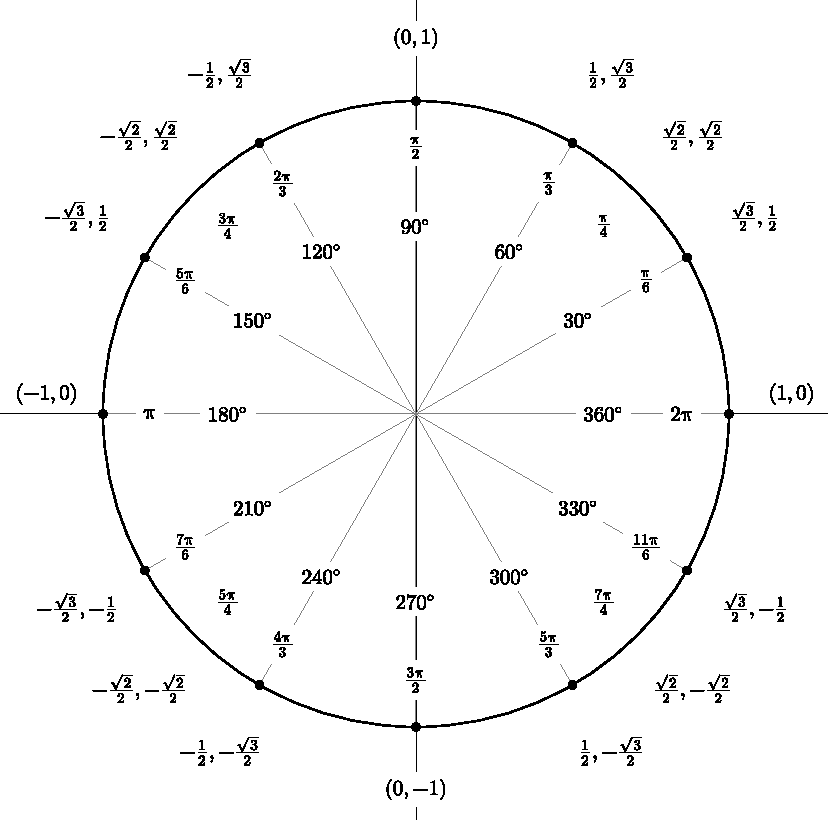
\includegraphics[scale=0.5]{build/pictures/degrees_circle.pdf} 


\end{flushleft}


   \end{multicols}






\begin{tabular}{|c|c|c|c|c|}
  \hline
  Function & $x_0$ & $T_{\infty}$ & Constraints & First Terms \\
  \hline
  $\sin(x)$ & $0$ & $\sum_{n=0}^{\infty}(-1)^n \frac{x^{2n+1}}{(2n+1)!}$ & & $x - \frac{x^3}{6}+\frac{x^5}{120}-\frac{x^7}{5040}+\frac{x^9}{362880} \ldots$ \\
  \hline
  $\cos(x)$ & $0$ & $\sum_{n=0}^{\infty}(-1)^n \frac{x^{2n}}{(2n)!}$ & & $1- \frac{x^2}{2}+\frac{x^4}{24}-\frac{x^6}{720}+\frac{x^8}{40320} \ldots$ \\
  \hline
  $\tan(x)$ & $0$ & $\sum_{n=1}^{\infty} \frac{B_{2 n}(-4)^n\left(1-4^n\right)}{(2 n) !} x^{2 n-1}$ & & $x+\frac{x^3}{3}+\frac{2 x^5}{15}+\frac{17 x^7}{315}+\frac{62 x^9}{2835} \ldots$ \\
  \hline
  $\arccos(x)$ & $0$ & $\sum_{n=0}^{\infty} \frac{(2 n) !}{4^n(n !)^2(2 n+1)} x^{2 n+1}$ & $|x|<1$ & $x-\frac{x^3}{3}+\frac{x^5}{5}-\frac{x^7}{7}+\frac{x^9}{9} \ldots$ \\
  \hline
  $\arcsin(x)$ & $0$ & $\frac{\pi}{2}-\arccos(x)$ & $|x|\leq1$ & $\frac{\pi}{2}-\left(x-\frac{x^3}{3}+\frac{x^5}{5}-\frac{x^7}{7}+\frac{x^9}{9}\right) \ldots$ \\
  \hline
  $\arctan(x)$ & $0$ & $\sum_{n=0}^{\infty}(-1)^n \frac{1}{2 n+1} x^{2 n+1}$ & $|x|\leq1$ & $x-\frac{x^3}{3}+\frac{x^5}{5}-\frac{x^7}{7}+\frac{x^9}{9} \ldots$ \\
  \hline
  $e^{x+c}$ & $0$ & $\sum_{n=0}^{\infty} \frac{(x)^n}{n!}$ & & $1 + x + \frac{x^2}{2} + \frac{x^3}{6} + \frac{x^4}{24} \ldots$ \\
 
  \hline
  $\ln(x)$ & $1$ & $\sum_{n=1}^\infty \frac{(-1)^{n+1}}{n}(x-1)^n$ & $0< x \leq 2$ & $(x-1) - \frac{(x-1)^2}{2} + \frac{(x-1)^3}{3} - \frac{(x-1)^4}{4} + \frac{(x-1)^5}{5} \ldots$ \\
  \hline
  $\ln(1+x)$ & $0$ & $-\sum_{n=1}^{\infty}\frac{x^n}{n}$ & & $x- \frac{x^2}{2}+\frac{x^3}{3}-\frac{x^4}{4}+\frac{x^5}{5} \ldots$ \\
  \hline

  $\sqrt{x+1}$ & $0$ & $-\sum_{n=0}^{\infty}\binom{\frac{1}{2}}{n}x^n$ & & $1 + \frac{x}{2}-\frac{x^2}{8}+\frac{x^3}{16}-\frac{5x^4}{128} \ldots$ \\
  \hline
  $\frac{ax}{(b-x)^2}$ & $0$ & $\sum_{n=1}^{\infty}\frac{n \cdot x^n }{b^{n+1}}$ & & $\frac{ax}{b^2}+\frac{2ax^2}{b^3}+\frac{3ax^3}{b^4}+\frac{4ax^4}{b^5}+\frac{5ax^5}{b^6} \ldots$ \\
  \hline
\end{tabular}





\end{document}